\documentclass[12pt]{article}
\usepackage[margin=1in]{geometry}
\usepackage[svgnames]{xcolor}
\usepackage[utf8]{inputenc}
\usepackage{graphicx}
\usepackage{setspace}
\usepackage{hyperref}
\usepackage[colorinlistoftodos]{todonotes}
\usepackage{scrextend}
\usepackage{nameref}
\usepackage{mathtools}
\usepackage{fancyhdr}
\usepackage{indentfirst}
\usepackage{amsmath}
\usepackage{amsfonts}
\usepackage{amssymb}
\usepackage{enumerate}
\usepackage{ragged2e}
\usepackage{marginnote}
\usepackage{float}
\usepackage{marvosym}
\usepackage{listings}
\usepackage{tcolorbox}
\usepackage{wrapfig}
\usepackage{lipsum}
\tcbuselibrary{skins}
\tcbuselibrary{breakable}
\usetikzlibrary{decorations.pathmorphing}
\hypersetup{
colorlinks = true,
urlcolor = red
}
\doublespacing
\numberwithin{equation}{section}
% Def a global settings for box styles:
\tcbset{
	style_pic/.style={ beamer,colback=Honeydew!50!white,colframe=LightGray},
	style_eq/.style={beamer,breakable,colback=DarkGoldenrod!37},
	style_theo/.style={breakable,beamer,frame style={left color=red!75!black,right color=blue!75!black},interior style={left color=LightCoral!35!Azure,right color=Azure!60!AliceBlue} ,fonttitle=\bfseries, opacityback=0.95, titlerule=2pt,},    
	style_def/.style={beamer,breakable,enhanced,colback=Lavender!50,colframe=LightSteelBlue!70,colbacktitle=DarkSeaGreen!75!black,fonttitle=\bfseries,borderline north={3pt}{-1.5pt}{Navy!20!white,decoration={zigzag,amplitude=2pt},decorate},borderline south={3pt}{-1.5pt}{Navy!20!white,decoration={zigzag,amplitude=2pt},decorate},boxrule=0pt,sharp corners,toprule=1.25mm,bottomrule=1.25mm},
	style_lemma/.style={beamer,breakable,colframe=FireBrick!55!Black,interior style={top color=LightSalmon!40!white,bottom color=MintCream!30!white},fonttitle=\bfseries},
	style_coro/.style={beamer,breakable,colframe=Aqua!50!black,interior style={top color=LightBlue!70!,bottom color=MintCream},fonttitle=\bfseries},
	style_proof/.style={beamer,breakable,title=Proof,breakable,enhanced,skin=enhancedlast jigsaw,attach boxed title to top left={xshift=-4mm,yshift=-0.5mm}, fonttitle=\bfseries\sffamily,interior style={top color=MediumPurple!45!white,bottom color=DeepSkyBlue!15!white}, boxed title style={empty,arc=0pt,outer arc=0pt,boxrule=0pt}, underlay boxed title={ \fill[BlueViolet!85!White] (title.north west) -- (title.north east)-- +(\tcboxedtitleheight-1mm,-\tcboxedtitleheight+1mm)-- ([xshift=4mm,yshift=0.5mm]frame.north east) -- +(0mm,-1mm)-- (title.south west) -- cycle;\fill[Indigo] ([yshift=-0.5mm]frame.north west)-- +(-0.4,0)--+(0,-0.3)--cycle;
			\fill[Indigo] ([yshift=-0.5mm]frame.north east)-- +(0,-0.3) -- +(0.4,0) -- cycle; }}
}

% Def a box for picture:
\newtcbox[auto counter, number within=section]{\picbox}[2][]{style_pic,title=Figure \thetcbcounter:~#2,label=pic:\thetcbcounter,#1}
% Def new command:
\let\bb\mathbb
\newcommand{\tincludegraphics}[3][]{\center\picbox{#3}{\includegraphics[width=310pt,#1]{#2}}}
% Def theorem environment:
\newtcolorbox[auto counter,number within=section]{box_for_theo}[2][]{style_theo,title=Theorem \thetcbcounter:~#2,label=th:\thetcbcounter,#1}


\newenvironment{theo}[2][]{\begin{box_for_theo}[#1]{#2}}{\end{box_for_theo}}

% Def lemma environment:
\newtcolorbox[auto counter, number within=section]{box_for_lemma}[2][]{style_lemma,title=Lemma \thetcbcounter:~#2,label=le:\thetcbcounter,#1}

\newenvironment{lem}[2][]{\begin{box_for_lemma}[#1]{#2}}{\end{box_for_lemma}}

% Def corollary environment:
\newtcolorbox[auto counter, number within=section]{box_for_coro}[2][]{style_coro,title=Corollary \thetcbcounter:~#2,label=co:\thetcbcounter,#1}

\newenvironment{coro}[2][]{\begin{box_for_coro}[#1]{#2}}{\end{box_for_coro}}

% Def definition environment:
\newtcolorbox[auto counter,number within=section]{box_for_def}[2][]{style_def,title=Definition \thetcbcounter:~#2,label=def:\thetcbcounter,#1}

\newenvironment{defi}[2][]{\begin{box_for_def}[#1]{#2}}{\end{box_for_def}}

% Def proof environment:
\newtcolorbox{box_for_proof}{style_proof}

\newenvironment{proof}{\begin{box_for_proof}}{\end{box_for_proof}}
% Def Equation environment:
\newenvironment{eq}[2][]{\begin{equation}\tcboxmath[style_eq,label=eq:#1]{#2}}{\end{equation}}

% Def general environment:
\newtcolorbox[auto counter,number within=section]{box_for_gene}[2][]{style_theo,title=\thetcbcounter:~#2,label=#1}


\newenvironment{general}[2][]{\begin{box_for_gene}[#1]{#2}}{\end{box_for_gene}}

% header and footer:
\pagestyle{fancy}
\rhead{\textbf{\thepage}}
\chead{}
\lhead{}
\lfoot{}
\cfoot{}
\rfoot{}
\renewcommand{\headrulewidth}{0pt}

% customized command:
\let\bb\mathbb
\newcommand{\suppose}{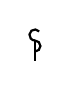
\begin{tikzpicture}[scale=0.35,thick]
		
		\draw (1.55mm,-0.7mm)arc (40:270:2mm);
		\draw (-0mm,-8mm)arc (270:450:2mm);
		\draw (0,-4mm)--(0,-11.5mm);
\end{tikzpicture} }

% add bibliography file and config:
\usepackage[backend=bibtex, sorting=ydnt, bibstyle=ieee]{biblatex}
\addbibresource{refs.bib}
\begin{document}
	
	\begin{titlepage}
		\hspace{0pt}
		\vfill
		\begin{tcolorbox}[style_def]
			\begin{center}
				\rule{\textwidth}{1.5pt}\\[1mm]
				\LARGE{\textbf{Point Distribution On The Sphere}}\\[3mm]
				\large{\textbf{Final edition}}\\[1mm]
				\rule{\textwidth}{1.5pt}\\[1mm]
			\end{center}
		\end{tcolorbox}
		\vfill
		\begin{tcolorbox}[style_pic]
			\begin{center}
				\large{Name: \textbf{Richard Lu}}\\
				\large{Report version: \textbf{1.5}}\\
				June 18, 2022
			\end{center}
		\end{tcolorbox}
	\end{titlepage}
	%\abstract{}
	%\thispagestyle{empty}
	%\clearpage
	\tableofcontents
	\thispagestyle{empty}
	\clearpage
	\setcounter{page}{1}

	\part{voronöi cell}
	
	\newpage
	\section{Introduction}
		This is a research report regarding to the study of `point distribution on the sphere'. this subject has been greatly studied by many researchers so far. Many important and beautiful results were presented over the years. While in this report, we try to follow the path of Dr. Han in his paper (see Section 2 in \cite{xiaolong_uniformly}
		).
		 The goal is to investigate the existence of  point distribution that satisfied those 3 sub-conditions as he (Dr.Han) mentioned in his paper (see Condition 4 in Section 2). \par
		 Many comments will be included and will be removed as the study progresses. One comments example is: 
		 
		 \vspace{10mm}
		\todo[inline]{this is an example of the comment}
		\par
		A discussion of the Tammes's problem and his dual problems will be included in the first part of this report, followed by a detailed exploration of the 3 sub-conditions mentioned above. The discussion of voronöi cell will be excluded in the first few version of this report.\par
		Here are some special notations used in this reports:\\
		
		
		\begin{tabular}{|c|c|}
			\hline 
			$\bb{T}_n$ & n-points distribution generated by solution of the n-points Tammes's problem \\
			\hline 
			dist(A, B) & the geodesic distance from point A to point B \\
			\hline
			\suppose & suppose that \\
			\hline 
			\Lightning & contradiction \\
			\hline
			$\bb{D}_n$ & n-points distribution generated by group-theoretic construction method in \cite{lubotzky_1986_hecke} \\
			\hline
		\end{tabular}
		
	\newpage
	\section{voronöi cell}
		In this section, a concise introduction of voronöi cell will be given. one of the origin of the voronöi cell is when one consider the post office problem : \par 
		Consider a town has multiple post offices, how can we assign each residence a post office that reduce the cost of delivering. That is, only assign the closest post office to one residence.
		
		\begin{figure}
				\centering
				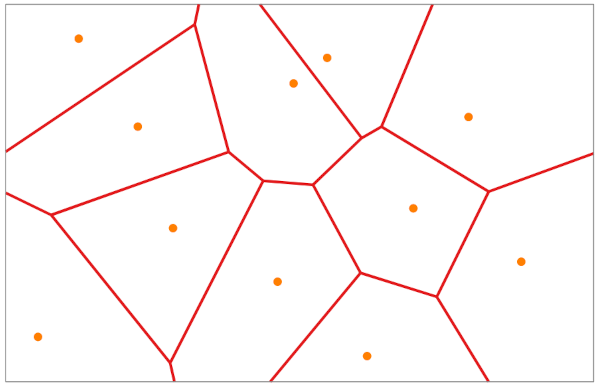
\includegraphics[width=0.7\linewidth]{vor1}
				\caption{voronöi cell example}
				\label{fig:vor1}
		\end{figure}

		As shown in the figure \ref{fig:vor1}, if we consider the each orange point as the post office. Then, the whole town could be partitioned into these small cells. Such that for any residence in the particular cell (i.e. any points in the cell), the closest post office to it is the cell site (the only post office in the cell). In this way, we preprocess the whole data points, and assign each data points to its closest cite. In the content of post office problem. We could pre-calculate the distance from every location on the map to the every post office and assign each residence with a particular location to its nearest post office. \par 
		One interesting application of the voronöi cell is that recent years, it has been used in the supervised classification algorithm in the area of machine learning. Many recommendation algorithms like nearest neighbour uses the voronöi network to make suggestions by finding the nearest (most similar) profile within a high dimensional space. \par 
		\subsection{Definition}
			It is time to formally define the voronöi cell:
			\vspace{5mm}
		\begin{general}[vor]{voronöi cell}
			For a given point set $\bb{P} = \{ P_1, P_2, P_3 \}$,
			The voronöi cell V($P_1$) $\coloneqq \{ x \in \bb{R}^n : |xP_1| < |xQ| \hspace{5mm} \forall Q\in \bb{P}  \backslash \{ P_1 \}\}$
		\end{general}
		
		On the other hand, if we define an auxiliary notion at first:
		 	\vspace{5mm}
		
		\begin{general}[half_plane]{half plane}
			For 2 points P, Q in some domain $\bb{D}$, the half plane is define as: \par 
			$h(P,Q) \coloneqq \{ x: |xP|<|xQ| \hspace{5mm} \forall x \in \bb{D} \}$
			
			 
		\end{general}
	
	if we adopt the above definition, voronöi cell could also be defined as follows:
	
		\begin{general}[vor2]{voronöi cell (alternative definition)}
			For a given point set $\bb{P} = \{ P_1, P_2, P_3 \}$,
			The voronöi cell V($P_1$) $\coloneqq \underset{P_1 \neq Q, \forall Q \in \bb{P}}{\bigcap} h(P_1, Q)$
			
			
		\end{general}
		
	Now, we have the voronöi cell, we could use it to finish another two related definition:
	\begin{general}[vor_edge]{voronöi edge}
		For a given point set $\bb{P} = \{ P_1, P_2, P_3 \}$,
			The voronöi edge V($\{P_1, P_2\}$) $\coloneqq $ relative-interior ($\partial V(P_1) \bigcap \partial V(P_2)$) $= \{ x: |xP_1| = |xP_2| \hspace{2mm}\& \hspace{2mm}|xP_1| < |xQ| \hspace{5mm} \forall Q\in \bb{P}\backslash \{P_1, P_2 \}   \}$
			
	\end{general}
	
	and finally, we have:
	
	\begin{general}[vor_vertex]{voronöi vertex}
		For a given point set $\bb{P} = \{ P_1, P_2, P_3 \}$,
			The voronöi vertex V($\{P_1, P_2, P_3\}$) $\coloneqq $ $\partial V(P_1) \bigcap \partial V(P_2) \bigcap \partial V(P_3)$ 
	\end{general}
	
	With all the finition above together (exclude Def \ref{vor2} and Def \ref {half_plane}), it creates a voronöi diagram system, denote as Vor($\bb{P}$) with a certain point set $\bb{P}$. For future reference, the point in this points set $\bb{P}$ are also called sites.
	
	\subsection{Basic Theorems}
		\begin{coro}[title = Theorem 1]{}
			Given a set $\bb{P} \subset \bb{R}^2 $ of n sites, Vor($\bb{P}$) consists of at most (2n-5) vertices and (3n-6) edges.
		\end{coro}
		
		
		\begin{proof}
			we start the proof by creating a dummy point A as shown in figure \ref{fig:pg1} \\
			Applying Euler characteristic equation we have: \par 
			$(|V|+1) - |E| +|F| = 2$ \par 
			$\Rightarrow$ $(|V|+1) - |E| + n = 2$ ($\alpha$) \\
			since every vertex has a degree $\geq$ 3\\
			$\Rightarrow$ $2|E| \geq 3(|V|+1)$\\
			$\Rightarrow$ $2\leq (|V|+1) + n -\frac{3}{2}(
			|V|+1)$\\
			$\Rightarrow$ $|V|+1 \leq 2n-4$\\
			$|V| \leq 2n-5 $ [plug in ($\alpha$) ] \\
			$\Rightarrow$ $|E|\leq 3n-6 $\\
			\begin{flushright}
				$\square$
			\end{flushright}
			
			
		\end{proof}
			You could access the planar graph used in the proof at:\par 
			\url{https://www.geogebra.org/calculator/rwdptfr8}
			
		\begin{figure}
			\centering
			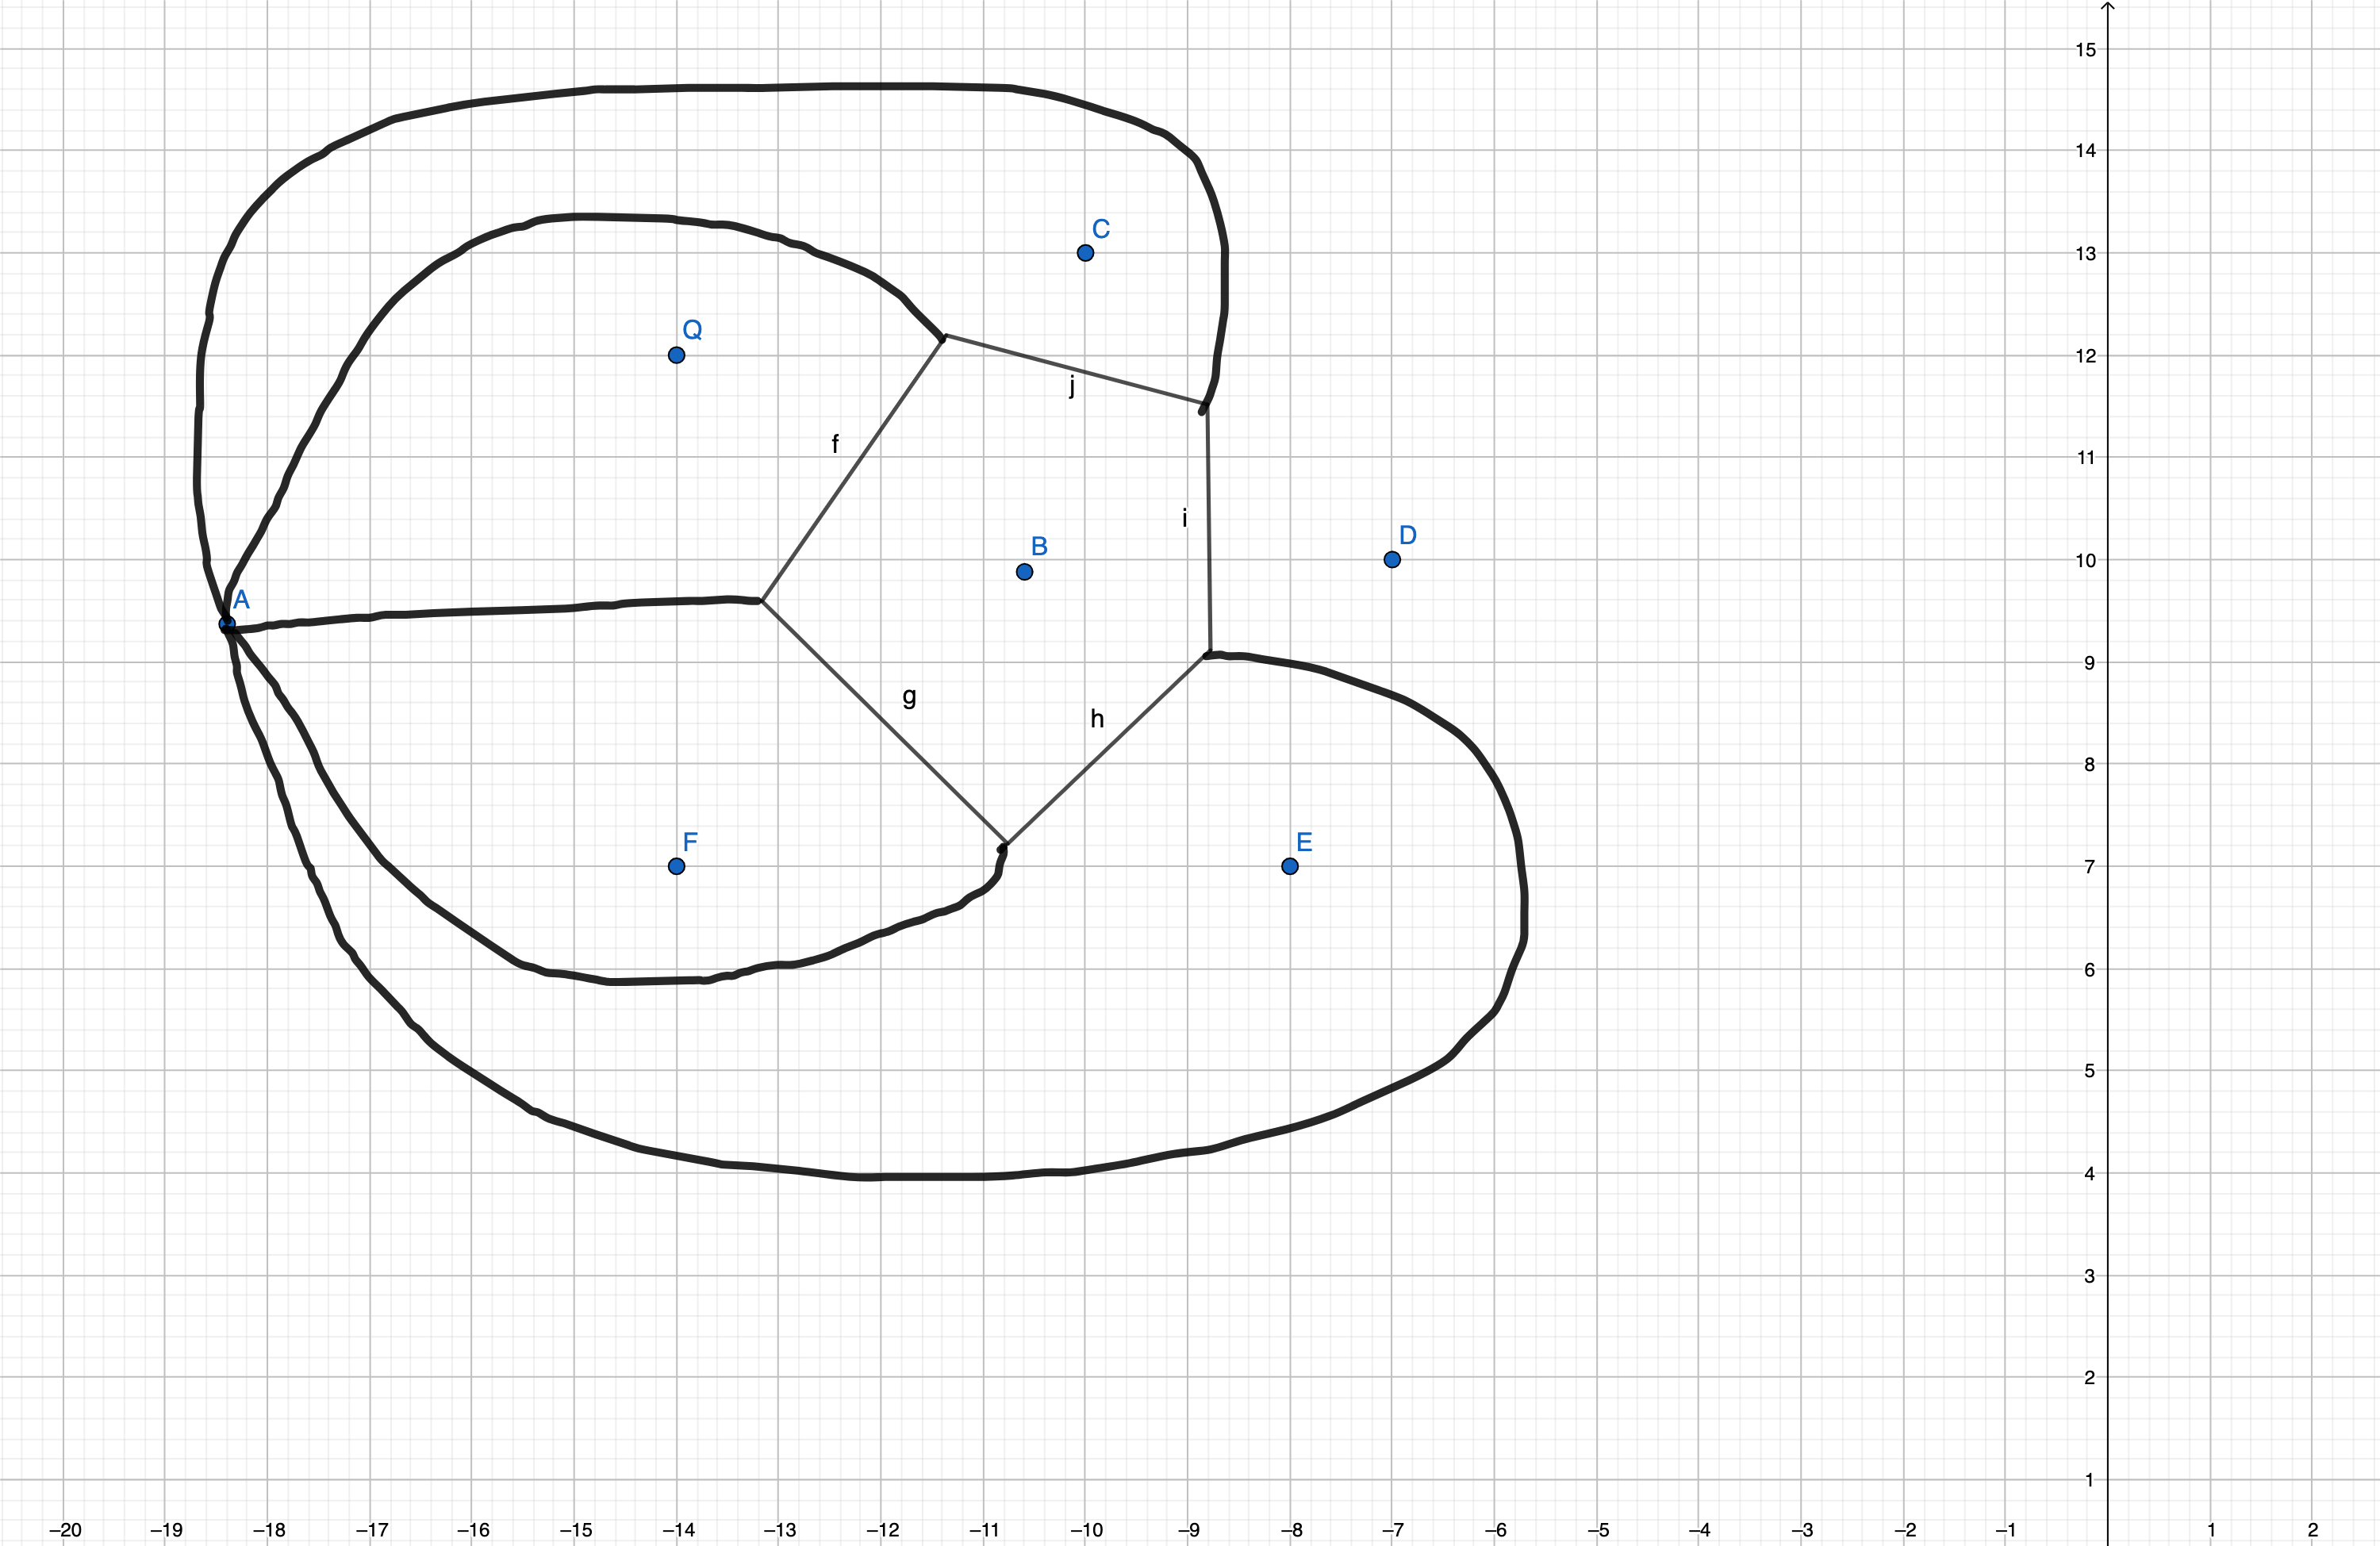
\includegraphics[width=1\linewidth]{theo1_planar_graph}
			\caption{planar graph}
			\label{fig:pg1}
		\end{figure}

		\vspace{10mm}
		
		\begin{coro}[title= Theorem 2]{}
			Let $\bb{P} \subset \bb{R}^2$ be a n-sites sets. If all sites are collinear, Vor($\bb{P}$) cosists only of (n-1) parallel lines. Otherwise, Vor($\bb{P}$) is connected and its edges are line segments or half-lines. 
		\end{coro}
		
		\begin{figure}
			\centering
			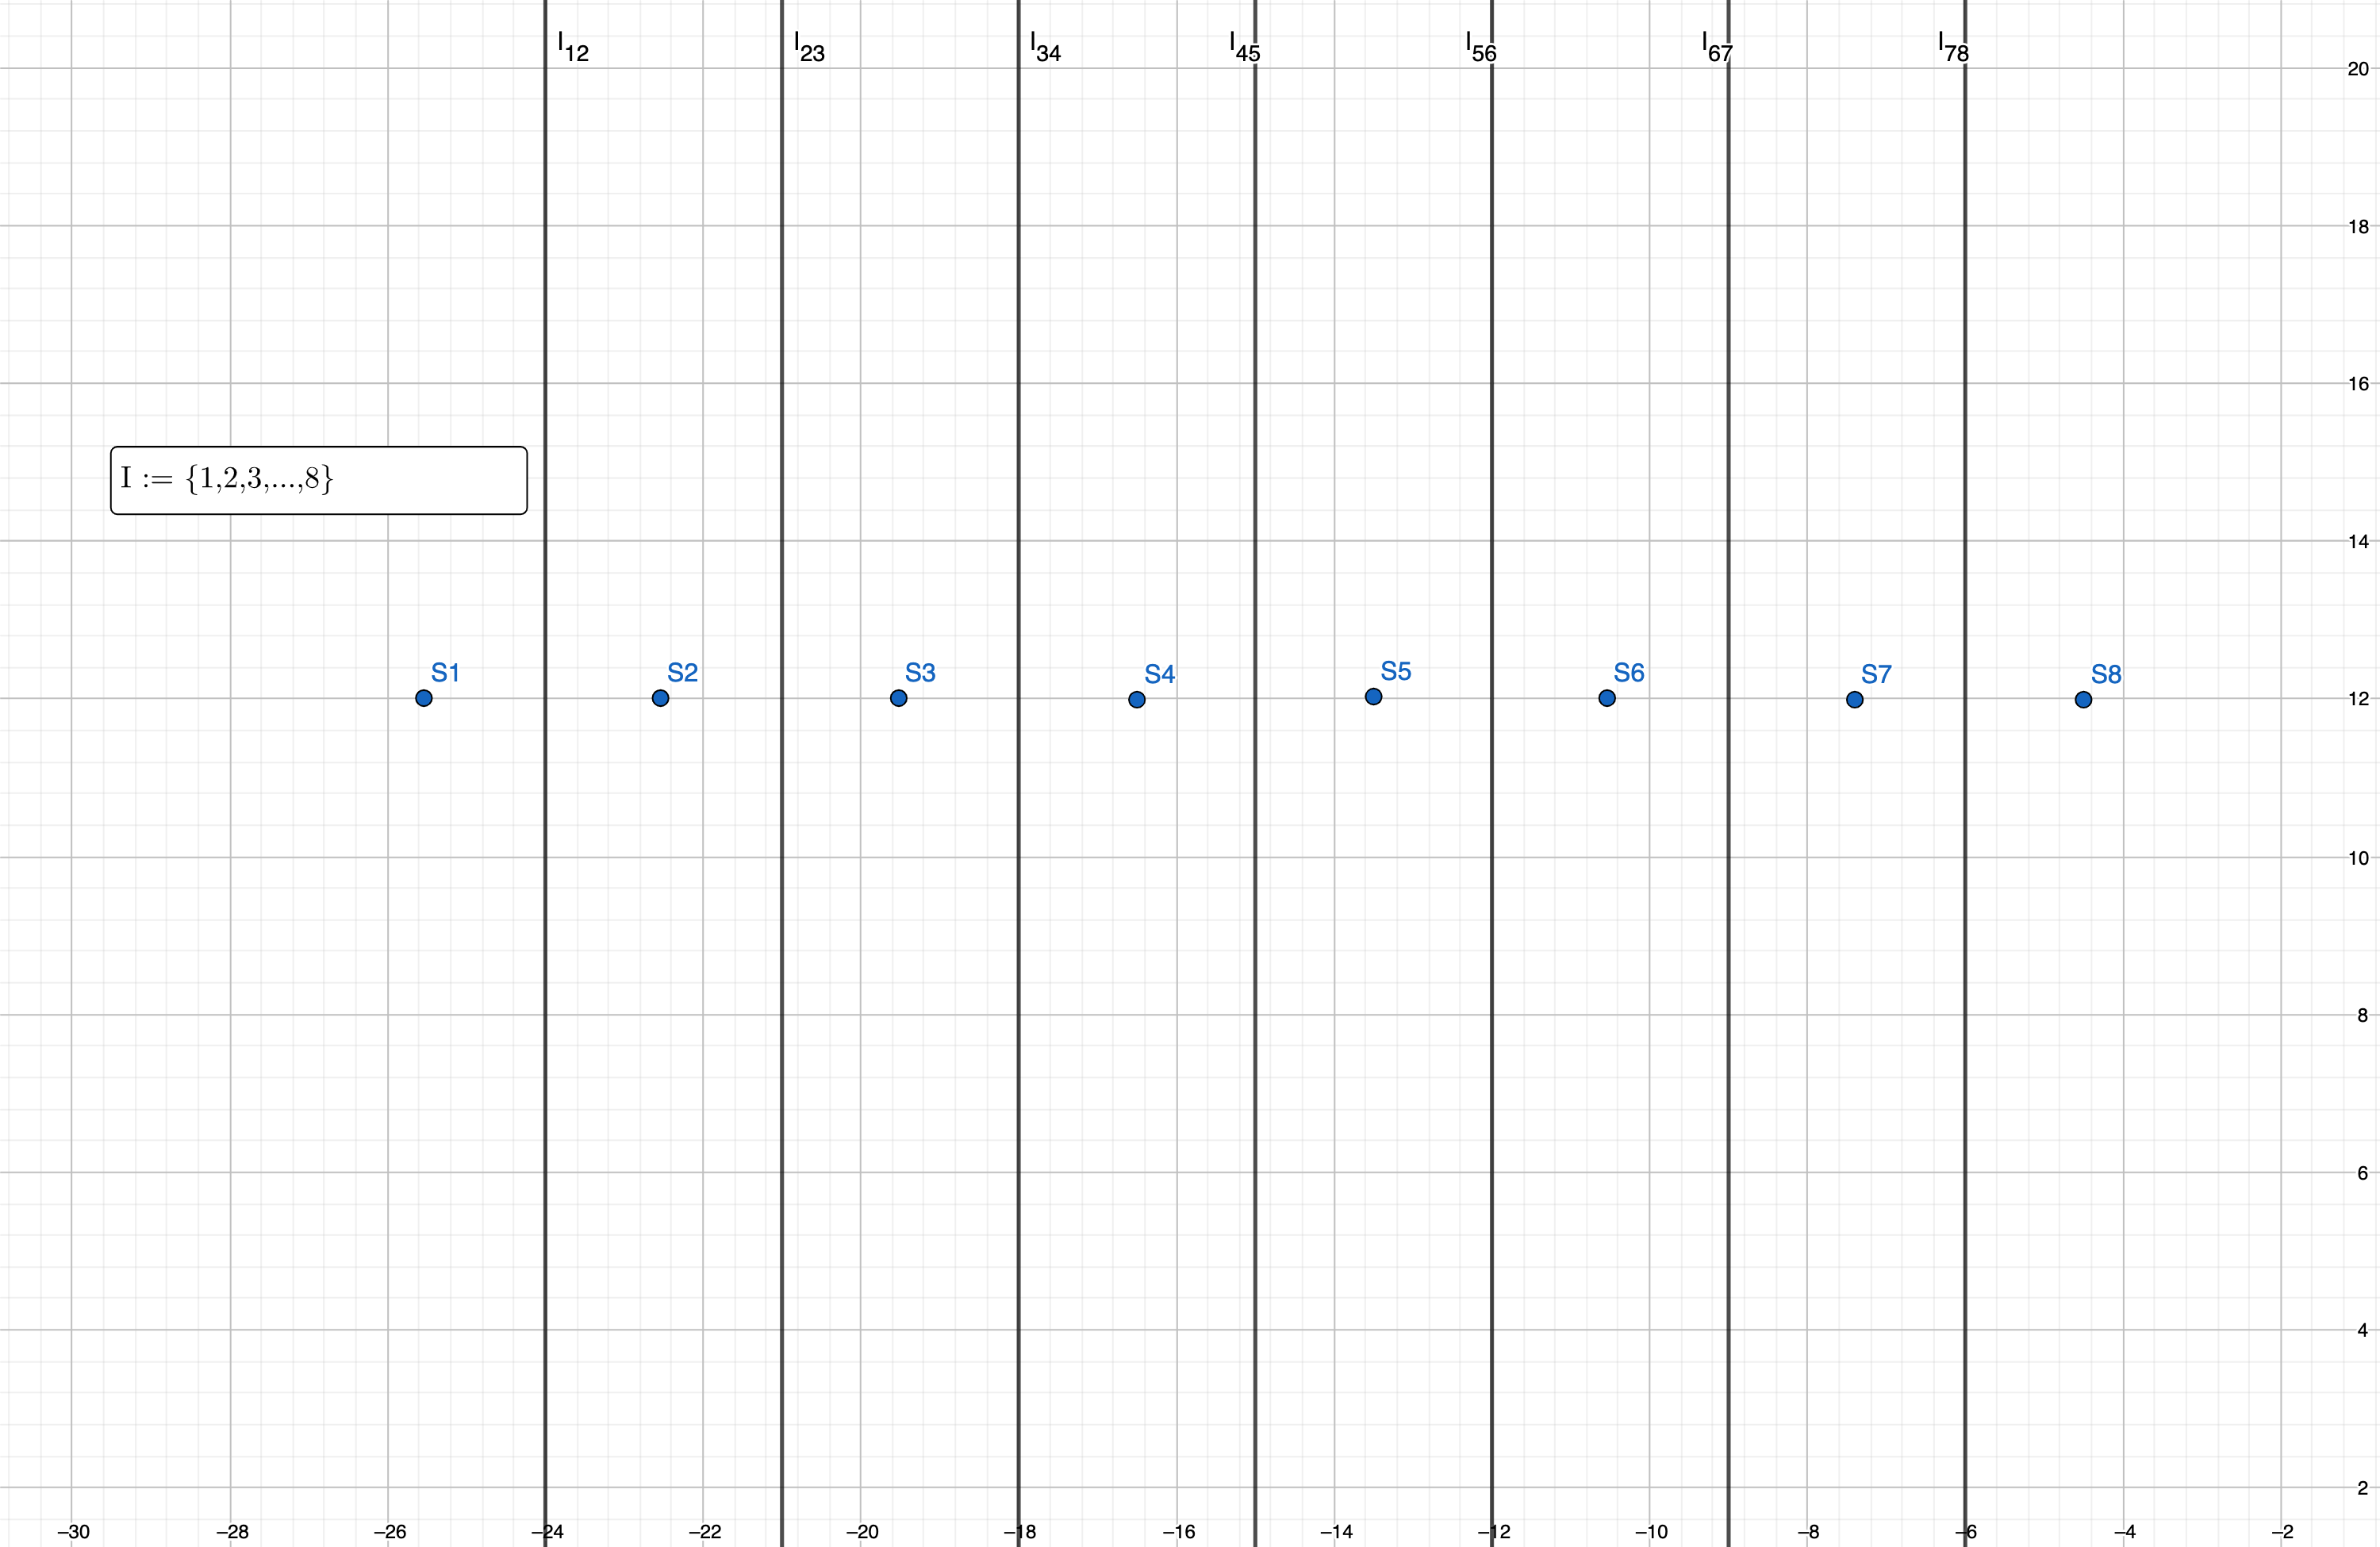
\includegraphics[width=0.9\linewidth]{theo2_vor}
			\caption{parallel lines}
			\label{fig:vor2}
		\end{figure}
		
		\begin{figure}
			\centering
			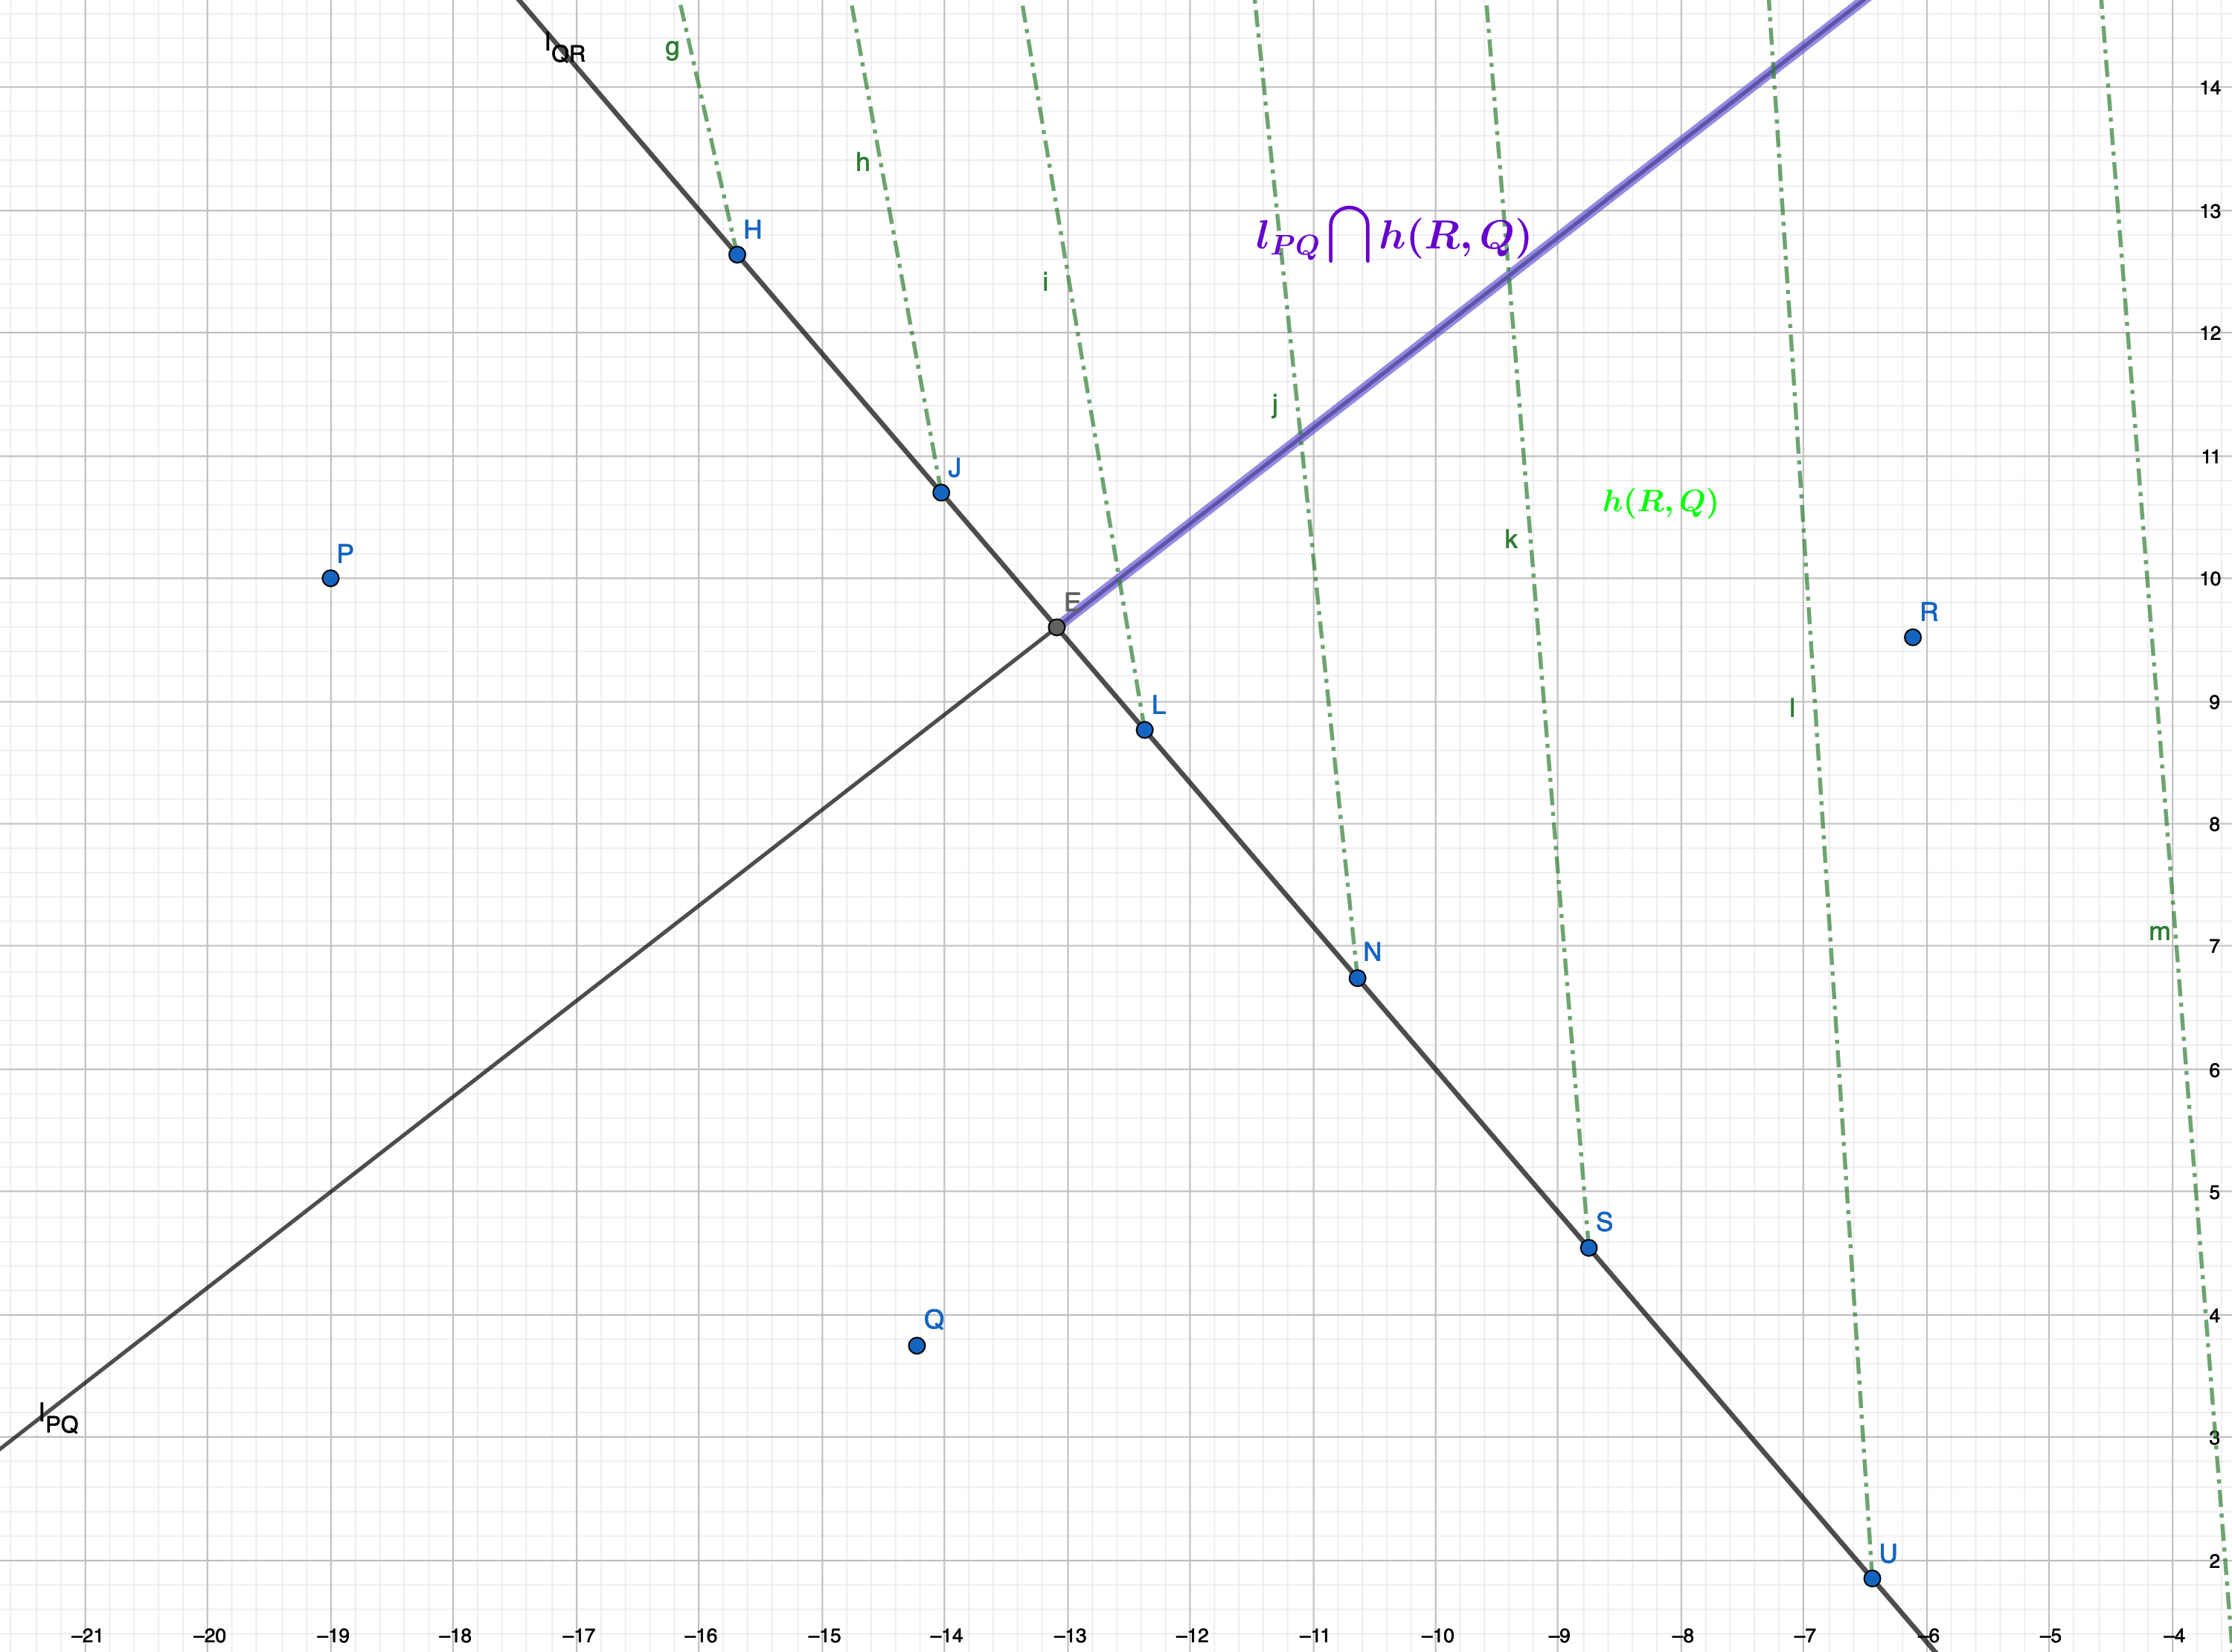
\includegraphics[width=0.9\linewidth]{theo2_vor2}
			\caption{Non collinear case}
			\label{fig:vor3}
		\end{figure}
		
		\begin{proof}
			The main proof contains 2 parts.
				\begin{enumerate}
					\item If all the sites are collinear, refer to the figure \ref{fig:vor2}. (This graph shows an example of 8 points, but it's also apply to n points)\\
					A first observation told us that there is no voronöi vertex in this graph. we shall proof this claim by contradiction.\\
					$\suppose $ there exists a voronöi vertex and this vertex is formed by $S_a, S_b, S_c \in  I$. \\
					if we denote this vertex as $V_0$, then it must satisfy:
					$|S_a V_0| = |S_b V_0| = |S_c V_0|$ \\
					Denote $V_{mn} \coloneqq \{V_0\in \bb{R}^2 : |S_mV_0| = |S_nV_0|\}$ for $m,n \in I$\\
					$\Rightarrow $ $V_0 \in V_{ab} \bigcap V_{bc}$\\
					however, 3 points already determines the center of the circle, which means:\\
					$\Rightarrow $ $V_0 = V_{ab} \bigcap V_{bc}$\\
					by definition, $V_ab$ is the bisection of points $S_a$ and $S_b$\\
					$\Rightarrow$ $V_ab = l_ab$ \\
					Similarly:\\
					$\Rightarrow V_bc = l_bc$ \\
					$\Rightarrow V_ab \parallel V_bc$\\
					$\Rightarrow$ $V_0 = V_{ab} \bigcap V_{bc} = \emptyset$\\
					By ruling out the possibility of voronöi vertices. It could only contain voronöi edges, with n cites, it generates (n-1) parallel voronöi edges.
					
					\item If not all the sites are collinear\\
						now refer to the figure \ref{fig:vor3}\\
						$\suppose \,\, \exists R \in \bb{P}$, R is not collinear with P and Q\\
						first by the definition of voronöi system, Vor$(\bb{P})$ is connected.\\
						now $\suppose$ \,\,\, $\exists $ a voronöi edge $l_{PQ}$ in Vor$(\bb{S})$ where $\bb{S}$ denotes the current sites.\\
						Assume that $l_{PQ}$ is a whole line (i.e. not a line segment)\\
						$\Rightarrow$ $\forall x\in h(R, Q)$, we have:
						$|xP|>|xR|, |xQ|>|xR|$\\
						Thus by the definition of the half plane $h(R, Q)$\\
						Some part of the line $l_{PQ}$ shouldn't be the edge of Vor($\bb{S}$)\\
						$\Rightarrow$ edge $l_{PQ}$ is not a whole line. It's bounded by $l_{QR}$ and it's either a line-segment or a half-line.
						
						
					
				\end{enumerate}
			
			\begin{flushright}
				$\square$
			\end{flushright}	
		\end{proof}
		
		you can access the figure \ref{fig:vor2} at \url{https://www.geogebra.org/calculator/kxdwsqry}
		and access figure \ref{fig:vor3} at \url{https://www.geogebra.org/calculator/ge9pgtub}
		
		Before proceeding to the Theorem 3, we need another definition about voronöi vertex.\\
		
		\begin{general}{Charaterization of voronöi vertex}
			$C_p(x) \coloneqq$ The largest circle centered at x without sites in its interior.
		\end{general}
		Now we are ready for the Theorem 3:
		\begin{coro}[title=Theorem 3]{}
			Let $\bb{P} \subset \bb{R}^2$ be a n-sites sets.\\
			if x is a voronöi vertex $\Leftrightarrow$ $|C_p(x) \bigcap \bb{P}| \geq 3$.
		\end{coro}
		
		\vspace{5mm}
		
		\begin{proof}
			\begin{enumerate}
				\item if x is a voronöi vertex $\Rightarrow$ $|C_p(x) \bigcap \bb{P}| \geq 3$\\
				if x is a voronöi vertex, by the definition. It must have 3 or more sites around it.\\
				i.e. $x = V(\{ P_1, P_2, P_3, ..., P_n \})$ with $P_n \in \bb{P}$, now use the definition 2.5:\\
				We get:\\
				$|xP_1| = |xP_2| = |xP_3| = ... = |xP_n|$\\
				This is an indication that $P_1,...,P_n$ are on the circle $\bigodot A$ which centered at $x$ with radius $|xP_1|$\\
				Now we have to proof $\bigodot A$ is the largest circle centered at $x$ without sites in its interior.\\
				$\suppose \,\, \exists Q \in \bb{P}\backslash \{P_1,...,P_n\}$, and assume it sits inside the $\bigodot A$, it means:\\
				$|xQ| < |xP_1|$\\
				However, by the definition of the voronöi vertex of $x$ regarding to site $P_1$, it must satisfy:\\
				$|xP_1| < |xM| \hspace{5mm} \forall M \in \bb{P}\backslash \{P_1,...,P_n\}$ \hspace{4mm} (\Lightning)
				
				
				\item if x is a voronöi vertex $\Leftarrow$ $|C_p(x) \bigcap \bb{P}| \geq 3$\\
					By the definition of $C_p(x)$, there is no sites in its interior, which means $C_p(x) \bigcap \bb{P}$ contains only the sites on the boundary of the circle $C_p(x)$. \\
					$\suppose $ $|C_p(x) \bigcap \bb{P}| = n \geq 3$, i.e. there are n points around the center $x$\\
					explicitly, assume these points are $P_1, P_2,...,P_n$. Since these points are on the boundary of the circle $C_p(x)$, we have:\\
					$|xP_1| = |xP_2| = |xP_3| = ... = |xP_n|$ \\
					also notice, there are no other sites in this circle, means:\\
					$|xP_1| < |xM| \hspace{5mm} \forall M \in \bb{P}\backslash \{P_1,...,P_n\}$\\
					together, we have:
					$x$ is a voronöi vertex of Vor($\bb{P}$)
					
			\end{enumerate}
			
			
			\begin{flushright}
				$\square$
			\end{flushright}
		\end{proof}
		
	\subsection{Fortune's Algorithm}
		The Fortune's algorithm is invented to generate the voronöi diagrams in 2 dimensional space. Explicitly, the Fortune's algorithm inputs n sites with a region D, It outputs the voronöi diagrams or deivided region $D'$ with multiple voronöi cells.\par 
		
		Before starting the introduction of this algorithm, two concepts must be introduced first. The whole algorithm is based on the sweeping line algorithm. it means that in this algorithm, it has a horizontal line (sweep line) moves from top to bottom, each time it hits a cite in the point distribution, the system triggers some events. As shown in Figure \ref{fig:fortune1}, The Sweep line L is the horizontal line that controls the whole process while the beach line is a monotone curve formed from the closet pieces of parabolic arcs (closest to the sweep line L)\\
		\begin{general}{fortune's algorithm}
			Given a region D and n sites.
			\begin{enumerate}
				\item Placing the Sweep line L above all the sites and start to move down slowly.
				\item Each time when L passes over a new site, trigger the point events.
				\item Additionally, when one parabolic arc shrinks to zero, trigger the circle events.
				\item As the sweep line L moving down to a point where no events can be triggered, stops the algorithm.
			\end{enumerate}
		\end{general}
		
		\subsubsection{Point events}
			As shown in figure \ref{fig:fortune3} whenever the point event are triggered, we first shoot a vertical ray up to the parabola that lies above this point in the beach line.Then split the arc into two parts by inserting a new small arc at this points. The newly created parabolic arc has the directrix L (same as the sweep line, we assume that the equation for L is simply: y = L) and focus $P \in \bb{P}$ ($P(P_x,P_y)$ is the site that L passes through.) And the arc has the equation: $(x-P_x)^2 = 2(P_y-L)[y-\frac{1}{2}(L+P_y)]$. Finally, as the sweep line goes down, the new arc will expand. Trace the intersection of different parabolic arcs on the beach line, we get the voronöi edges.
		\subsubsection{Circle events}
			Refer to figure \ref{fig:fortune4}, as the length of a parabolic arc shrinks to zero, then one of the parabolic arc on the beach line will disappear and a new voronöi vertex will be created at this special point.\par 
			A small proof to this events is that when one parabolic arc disappears as sweep line goes down as in the second graph in figure \ref{fig:fortune4}, if we denote this center point as $x$, then:\\
			$|xP_i| = |xP_j| = |xP_k|$, hence all three points lies on the same circle centered at $x$. Denote this circle by $C_p(x)$ and notice that there is no other cites in this circle. Thus, $C_p(x)\bigcap \bb{P} = 3$, Finally by the Theorem 3 in section 2.2, $x$ is a voronöi vertex.
		\subsubsection{Live graph}
		
		\begin{figure}
			\centering
			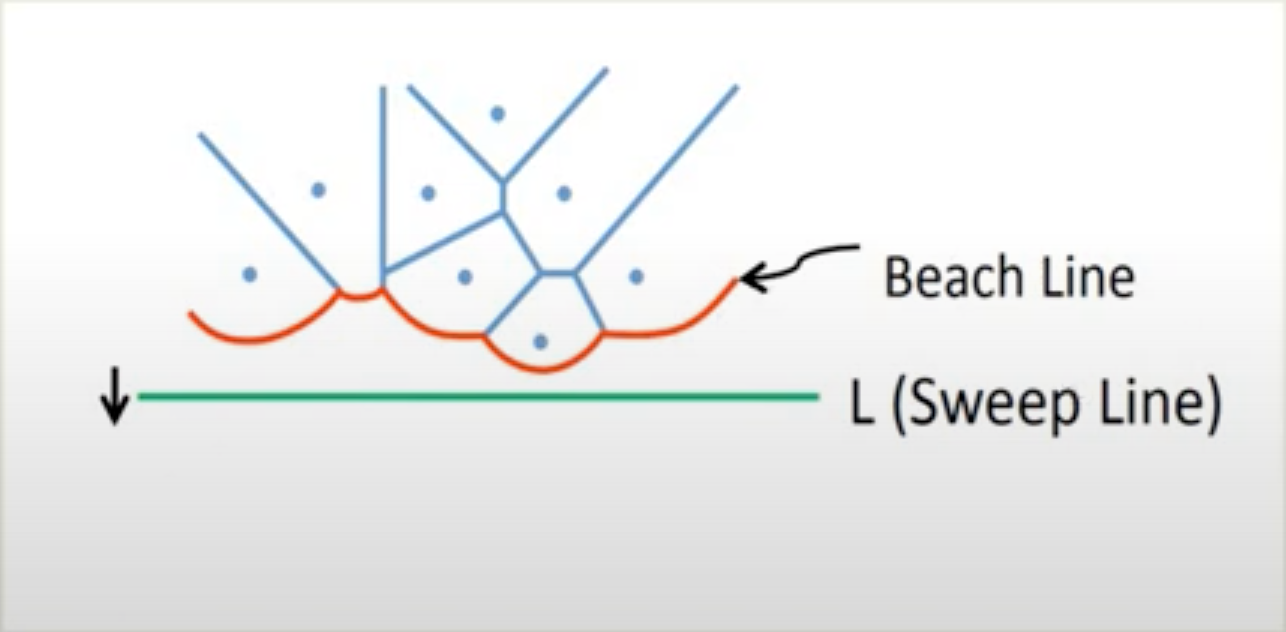
\includegraphics[width=0.7\linewidth]{fortune1}
			\caption{The sweep line and the beach line}
			\label{fig:fortune1}
		\end{figure}
		
		\begin{figure}
			\centering
			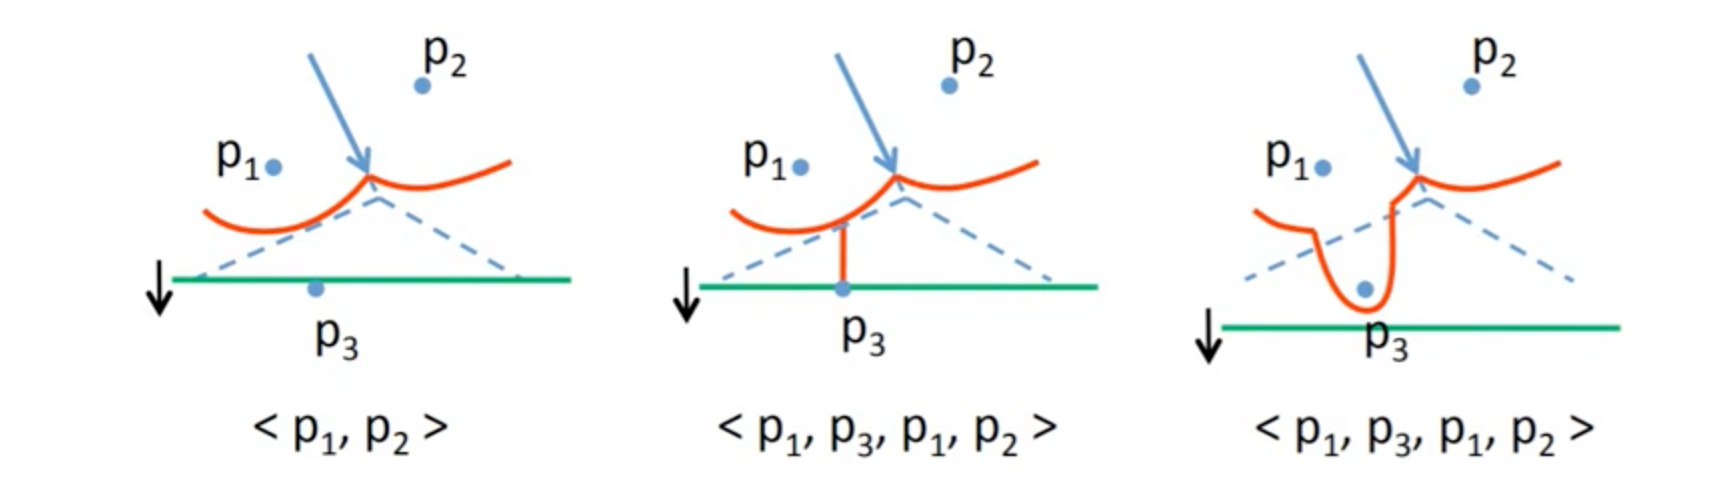
\includegraphics[width=0.7\linewidth]{fortune3}
			\caption{Point events}
			\label{fig:fortune3}
		\end{figure}
		
		\begin{figure}
			\centering
			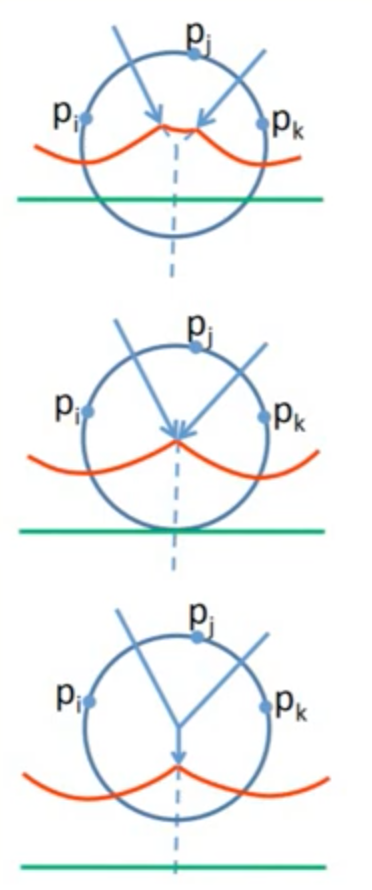
\includegraphics[width=0.2\linewidth]{fortune4}
			\caption{Circle events}
			\label{fig:fortune4}
		\end{figure}
		
		You could also access this live version of Fortune's Algorithm and play around with it: \\
		\url{https://www.desmos.com/calculator/ejatebvup4?lang=pl}
	
	
	\newpage
	
	\part{Tammes' problem and point distribution on the sphere}
	\newpage
	
	\section{Tammes's Problem}
	Here is an introduction to Tammes's problem and its dual problems. It turns out that Tammes's problem has several different dual problem and may lead to many different ways of calculation. \par 
	The Tammes's Problem is named after a Dutch botanist R.M.L. Tammes. He posed this problem when he observed arrangements of exit places on the surface of spherical pollen grains in 1930. The problem is to packing a given number of circles $n$ on the surface of a sphere such that the minimum distance between circles is maximized.\\
	One of the dual problem to the Tammes's problem is to find the the n-point distribution $\{\bb{P}\}_1^n$ (point configuration) that maximize the minimal distance between any different points in the distribution. If we denote such maximized distance as $d_n$, then: \par 
		$d_n = max\{min\{P_iP_j: 1\leq i<j\leq n\}\}$ \par 
		
		The connection between these two problems are considering the n-points are the centers of the $n$ circles in Tammes's prblem.\par 
	Unfortunately, after passing nearly a decades, although many researches are conducted regarding to this subject. Only few small $n$ has a full solution. For larger $n$, there is still no  solution to it.
	\vspace{10mm}

	
	\newpage
	
	\section{Condition 1: Well-separation}
		\begin{general}[c1]{Well-separation}
		There exist absolute constant c $>$ 0 such that for any positive integer n, there is a collection of points $\{ P_j^n \}_{j=1}^n$ such that 
		for any j, k = 1,\dots, n and j $\neq$ k, \\
		dist($P_j, P_k$) $\geq$ $\dfrac{c}{\sqrt{n}}$ \\
		For some constant c and $P_j, P_k \in \bb{P}_n$
		\end{general}

	\vspace{10mm}
	
		If we wish to verify the $\bb{T}_n \,\, \forall n\in \bb{N}$ for condition 1, it's sufficient to find the lower bound of the geodesic version of $d_n = max\{min\{P_iP_j: 1\leq i<j\leq n\}\}$ in the Tammes's Problem. Since they both represent the distance of any two points in the distribution.\\
		
		If we could successfully find its lower bound, and call it as $L_t$, then: (Assuming everything is in geodesic distance)\\
		$\Rightarrow$ $d_n = dist(P_j, P_k) \geq L_t \geq \frac{c}{\sqrt{n}}$\\
		$\Rightarrow \sqrt{n}L_t \geq c$
		 \\
		 since $\sqrt{n} \geq 1$ \\
		 $\Rightarrow \sqrt{n}L_t \geq L_t$,\\
		 Thus we only have to make $c \leq L_t$, this condition will be satisfied.
		
		However, there are plenty of upper bound for $\bb{T}_n$ with the famous Fejes-Toth upper bound found by Dr.L. Fejes-Toth in his early paper.(see \cite{mooers_1994_tammess}, 2) But we didn't find many things about its lower bound. The lower paper that mentions a little about his lower bound is in \cite{eb_1997_distributing}. But we connot verify its validity at this moment due to the lack of resources. Some further study need to be done related to this subject.
	\vspace{10mm}

	
	\newpage
	\section{Condition 2: No clustering around great circles}
	\begin{general}[c2]{No Clustering around great circles}
	There exist absolute constant C $>$ 0 such that for any positive integer n, there is a collection of points $\{ P_j^n \}_{j=1}^n$ such that 
		for any great circle G $ \subset  \bb{S}^2$,
		The cardinality of $ \{ j:dist_{{\bb{S}}^2} (G, P_j)\leq \dfrac{1}{n} \}$ is smaller or equal to a constant C. \\
		$\forall$ $P_j \in \bb{P}_n$
	\end{general}
	\subsection{Problem Analysis}
	In order to test this hypothesis with some point distribution, A rudimentary algorithm could be formed which consists the following 3 general steps: (Here we use the point distribution $\bb{T}_n$ as an example\par
	1. generate the representing coordinates of each points in $\bb{T}_n$
	\par
	2. Given a specific great circle G, find $dist_{{\bb{S}}^2} (G, P) \, \forall P \in \bb{T}_n$
	and compare the every one of them with $\dfrac{1}{n} $
	,then calculate how many of those geodesic distance is less than $\dfrac{1	}{n}$ and denote this number as $l_G$ \par 
	3. By varying the equation of great circle G, find M $\coloneqq$ max\{$l_G: \forall$ great circle G inside the unit sphere\} \newline  
	\todo[inline]{I'll first analyze the feasibility of the above 3 steps one by one in the following paragraph:}
	

		\subsubsection{Analysis of Step 1:}  \par
		\begin{enumerate}
			\item  $\bb{T}_2$ \par 
			It is hard to obtain the coordinates of each points in $\bb{T}_n$ even knowing the solution for n-Tammes's problem. 
			\par 
			Try to start with the simplest case with n=2. Since there are only 2 points, the minimum distance between any 2 points in the distribution is the distance of this two points. Mathematically, if we denote an arbitrary 2-point distribution as $\bb{P}_2$, then:
			\[  Min \{dist(P_i, P_j) \,  \forall P_i,P_j \in \bb{P}_2\} 
			=  dist(P_1, P_2)\,  \text{for distinct } \, P_1, P_2  \in \bb{P}_2  \]
			
			Hence, we only need to maximize the distance of $P_1 $ and $P_2$ to solve the Tammes's problem with 2 points.
			
			obviously:
			\par 
			$\bb{T}_2$ is the configuration where the 2 points are placed in the antipodal position on the sphere. \par
			
			WLOG, choose these 2 points to be the north and south pole on the sphere, we have the Cartesian coordinates for $ \bb{T}_2$:
			
			\begin{equation}
				\label{t2}
				\bb{T}_2 : (0,0,1) \, \& \, (0,0,-1)
			\end{equation}
			\item $\bb{T}_3$ \par 
			
			Things start to become complicated starting from n=3, Dr.L.Fejes-Toth has first found and proved these configuration in 1945 and many other modern proves are formulated by other researchers later on. One of the geometrical prove can be found in this paper (see \cite{antoniano_2019_the}, 76). They proved that $\bb{T}_3$ has the configuration such that the 3 vertices form an equilateral triangle and lie in 1 great circle in the sphere. \par 
			
			WLOG, choose 1 point to be the north pole and together with the other 2 points, they form a equilateral triangle in the x-z plane on the sphere: 
			
			\begin{equation}
				\label{t3}
				\bb{T}_3 : (0,0,1) , (-\dfrac{\sqrt{3}}{2}, 0, -\dfrac{1}{2}) , (\dfrac{\sqrt{3}}{2}, 0, -\dfrac{1}{2})
			\end{equation}
			
			The following graph is the graphical configuration for
			$\bb{T}_2$,$\bb{T}_3$,$\bb{T}_4$,$\bb{T}_5$,$\bb{T}_6$ respectively.
			\begin{figure}
				\centering
				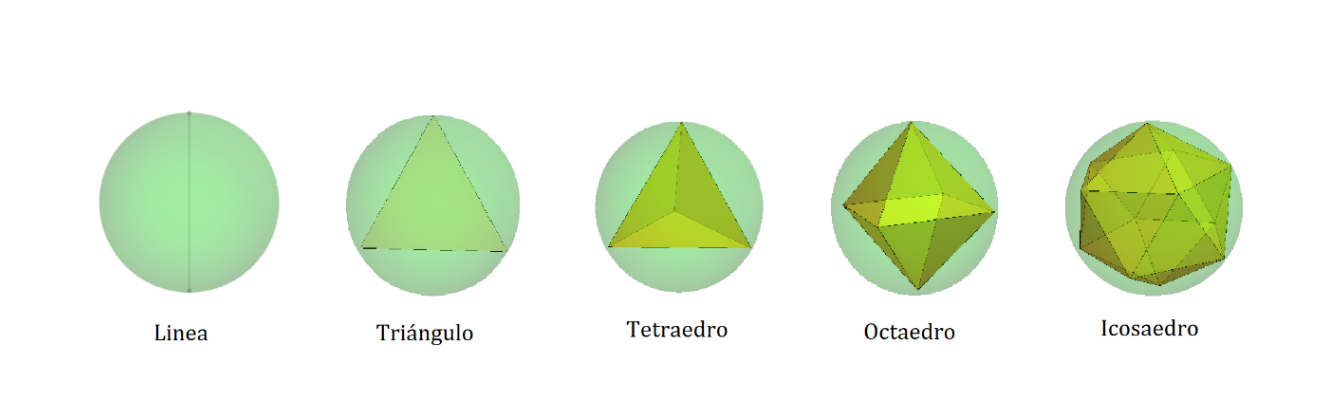
\includegraphics[width=0.7\linewidth]{T_n_Sol}
				\caption{Solutions for $\bb{T}_n$ (Antoniano, 2019)}
				\label{fig:tnsol}
			\end{figure}
			\newline
			\item $\bb{T}_4$ \par 
			The solution of 4-point Tammes's problem is more complicated but similar to $\bb{T}_3$ (see \cite{antoniano_2019_the} and \cite{mooers_1994_tammess}). They found the general configuration for $\bb{T}_4$ is a regular tetrahedral. \par 
			
			WLOG, choose 1 point of the tetrahedral to be the north pole, we could calculate the coordinates of rest of the points according to the Figure \ref{fig:tetrahedral} and get one of the possible representation:
			
						
			\begin{figure}
				\centering
				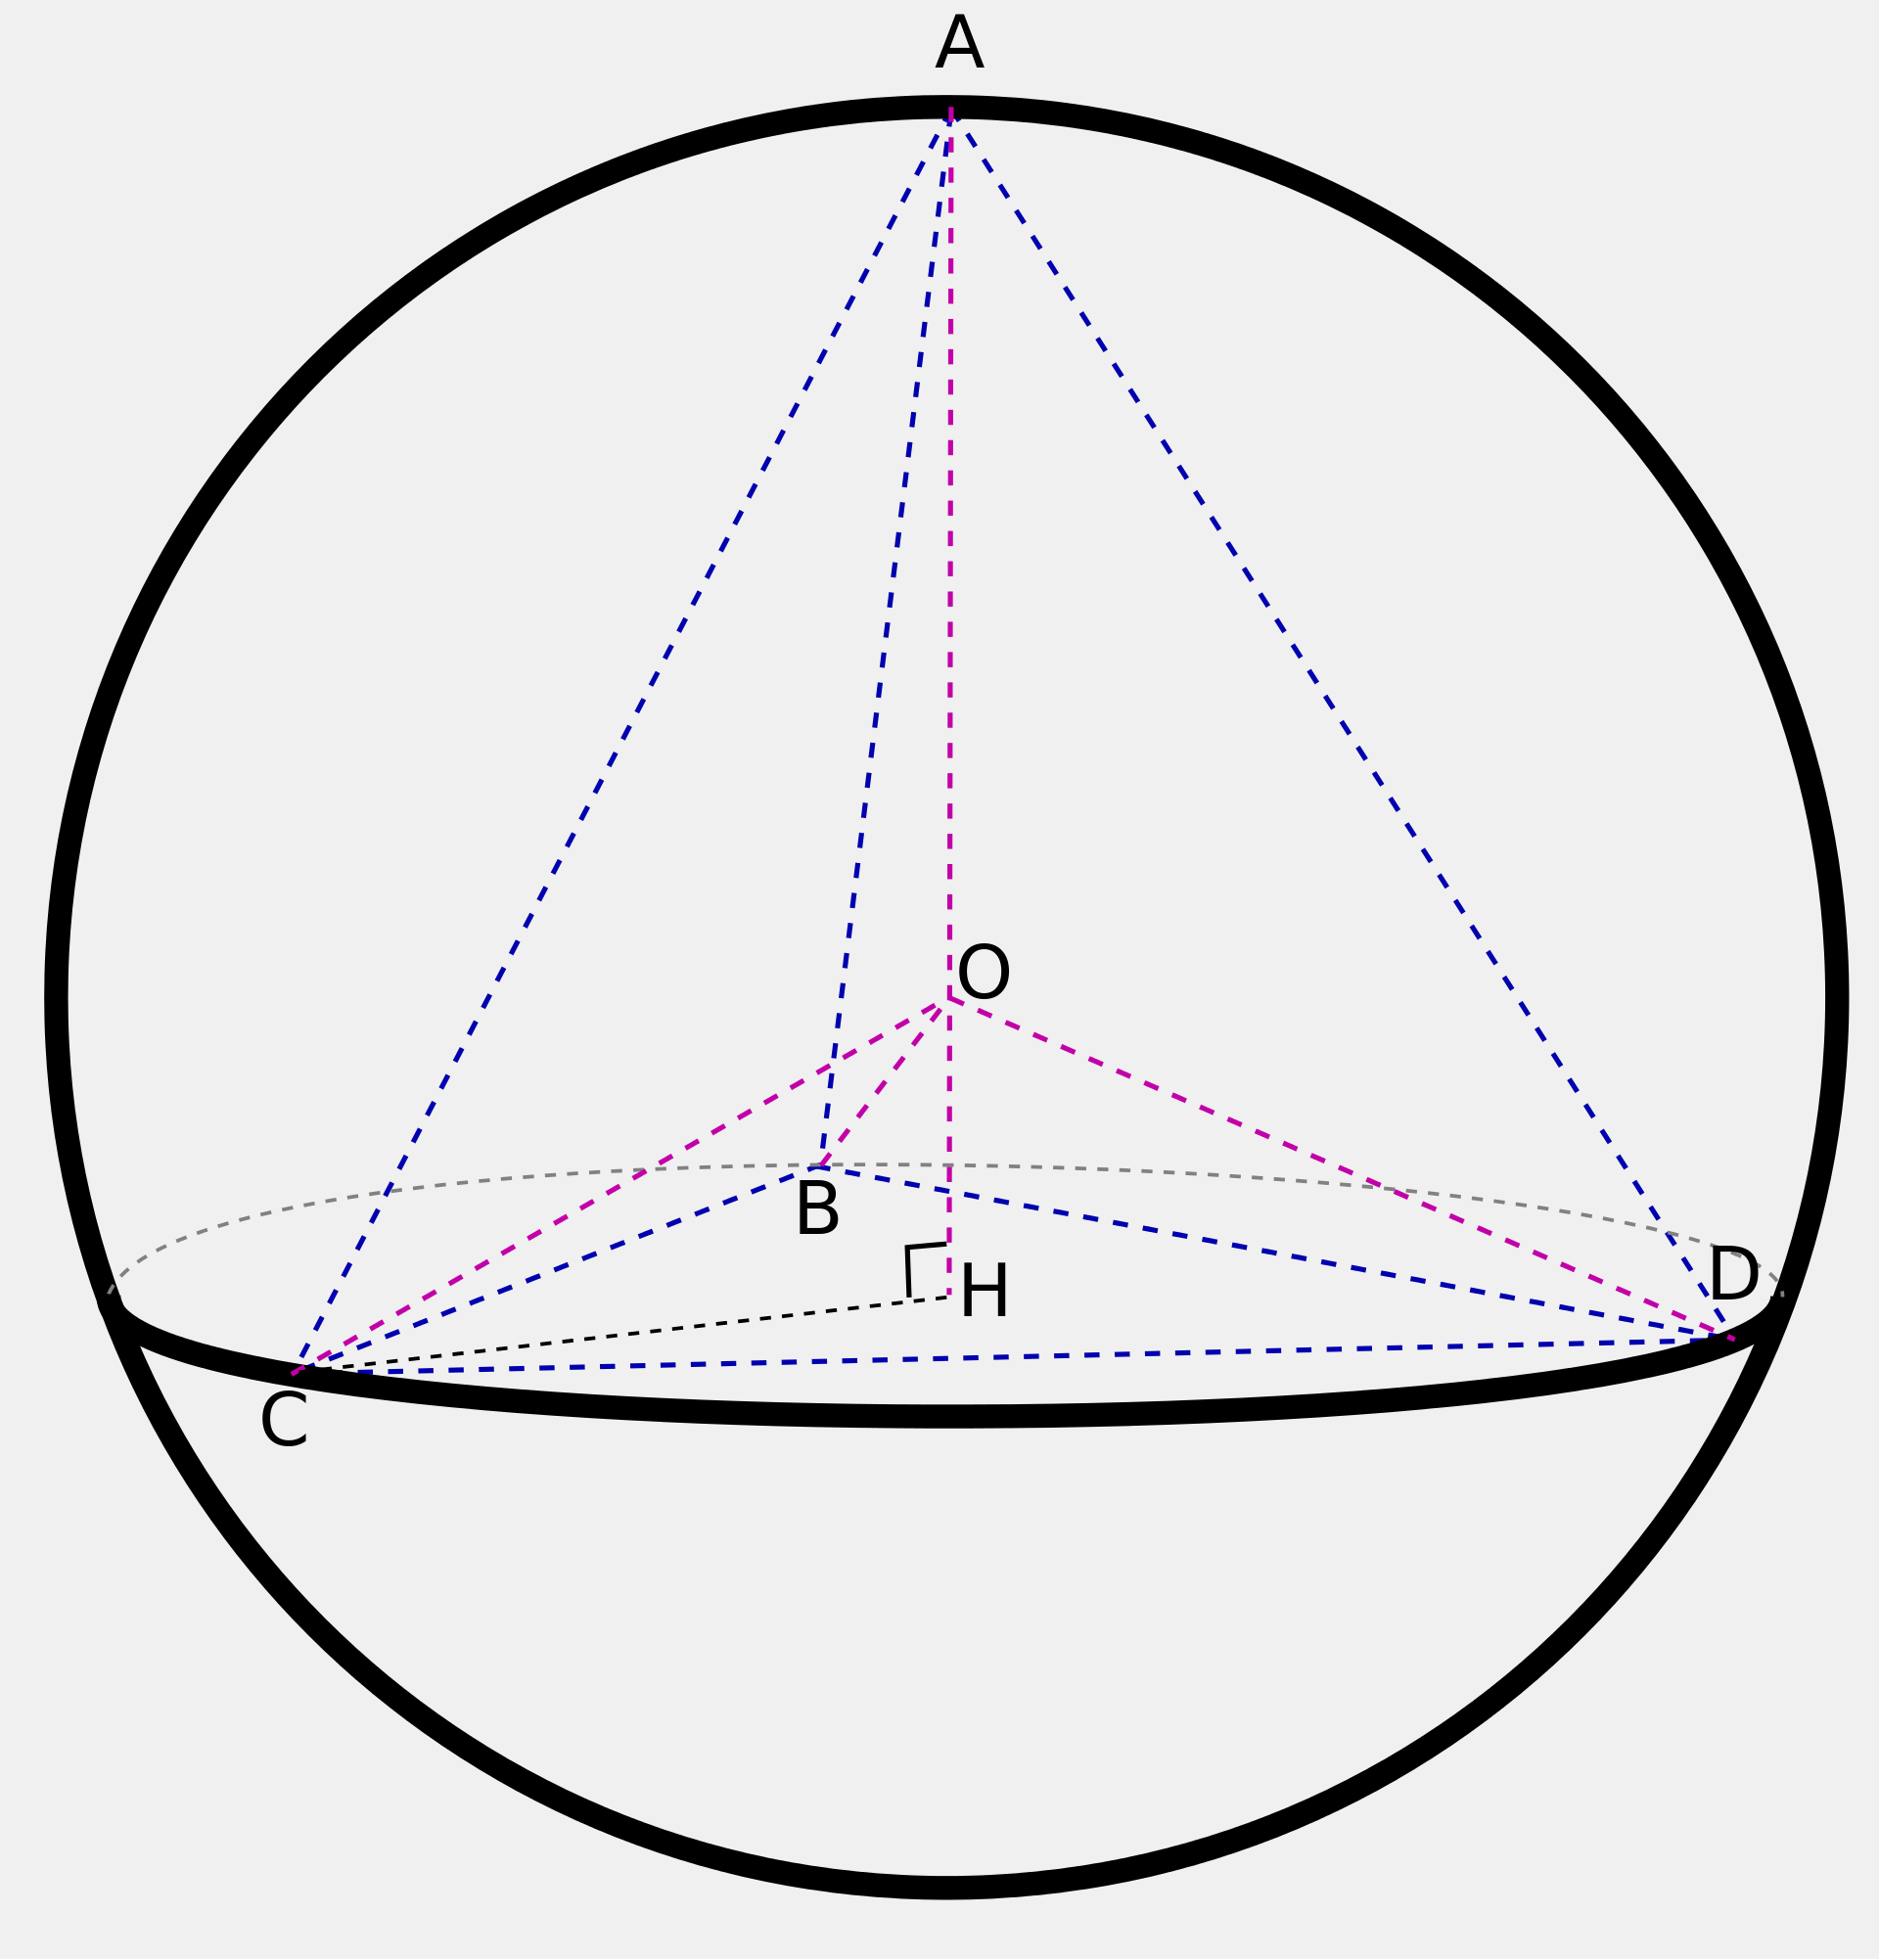
\includegraphics[width=0.5\linewidth]{tetrahedral}
				\caption{Tetrahedral}
				\label{fig:tetrahedral}
			\end{figure}
			
			
			
			
			\begin{equation}
			\label{t4}
			\bb{T}_4 : (0,0,1) , (0, \dfrac{\sqrt{3}}{2}, 	-\dfrac{1}{2}) , (\dfrac{3}{4}, -\dfrac{\sqrt{3}}{4}, -\dfrac{1}{2}), (-\dfrac{3}{4}, -\dfrac{\sqrt{3}}{4}, -\dfrac{1}{2})
			\end{equation}
		
		\todo[inline]{For higher n points, the solution is either non-regular or extremely hard to calculate. See \cite{sugimoto_2015_exact}, they spent most of their paper in calculating the exact coordinates of $\bb{T}_{10}$. there is only a numerical result in this paper and extremely hard to solve.}

		\vspace{10mm}
		\todo[inline]{There is a way that in general could give us a numerical solution for any $\bb{T}_n$, but the calculation takes days even weeks just for calculating $\bb{T}_n, \, \forall n \leq 100 $, see \cite{hars_2020_numerical} and \cite{hars_2020_numerical100} for detail.}
			
		\end{enumerate}
		
	\subsubsection{Analysis of Step 2:}  \par
		To achieve the goal in step 2, all we need to do is  calculating the geodesic distance from one point in  to G (G is not varying). For example, if we wish to calculate the distance from point A to the great circle lying in x-y plane in the Figure \ref{fig:greatcircle}. First, we have to find the orthogonal great circle to G. If the projection of A is lying on the diameter of the great circle G as shown in the Figure \ref{fig:greatcircle} (Projection of A is B). The orthogonal great circle is $\bigodot$ OCD lying in x-z plane. Generally, the orthogonal circle is formed by a great circle going through the point itself and across through the projection of the point. Then the desired geodesic distance is the geodesic distance from points to the intersection point.
		As an example, the desired geodesic distance in Figure \ref{fig:greatcircle}  is simply the arc ${AEC}$. In order to calculate it, we could connect the line between point A and its projection B. Hence, it's easy to see:
		\par 
		\begin{align*}
			\text{dist} (A, G) &= \overset{\Huge\frown}{AEC} \\
						&= r \times \angle{AOB} \\
						&= r \times \arcsin \dfrac{AB}{r} \\
						&= \arcsin AB \hspace{5mm} \text{(unit sphere, r=1)}
 		\end{align*}
		
		
		\begin{figure}
			\centering
			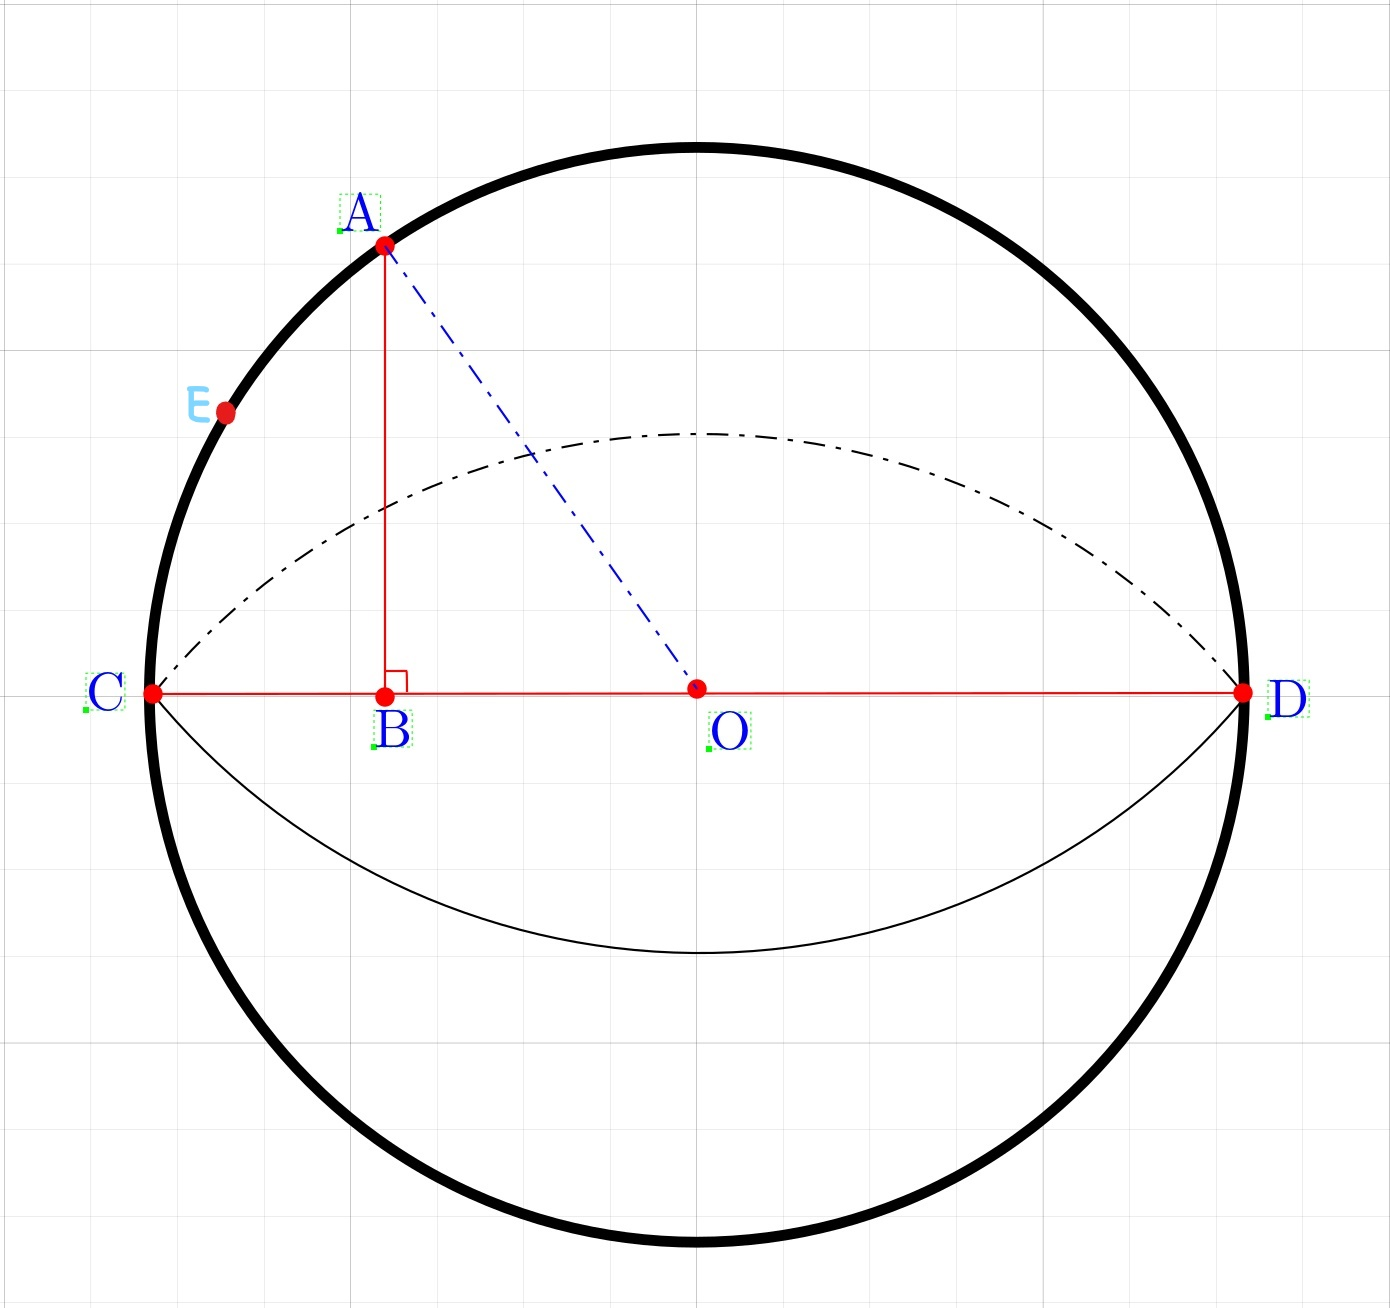
\includegraphics[width=0.5\linewidth]{great_circle_G}
			\caption{Great circle G is $\bigodot$ OCD lying in x-y plane}
			\label{fig:greatcircle}
		\end{figure}
		
		The above calculation applies to the general case as well. \par 
		Also notice, for some arbitrary great circle $G_a$ which lies in the plane $P:ax+by+cz=0$ (across through point$(0, 0, 0)$), we have: (with the same convention as above regarding to point A and B
		\par 
		
		\begin{align}
			\text{dist} (A, G_a) &= \arcsin AB \\
			&= \arcsin (dist_c(A, P)) \\
			&=\arcsin(\dfrac{|ax_A+by_A+cz_A|}{\sqrt{a^2+b^2+c^2}}) \label{dist}
		\end{align}
	
		where $\text{disc}_c$ denotes the normal Cartesian distance and point A has Cartesian coordinate $(x_A, y_a, z_a)$. \par 
		
		So far, we have obtained the explicit form of dist(A, G). But the biggest problem is about to come.
	\subsubsection{Analysis of Step 3:}  \par
		Based on the fact that we couldn't compare the dist(A, G) with $\dfrac{1}{n}$ from an arbitrary great circle G. the step 2 is theoretically impossible to finish. But if we consider the sum of all the distant from points to great circle G, denote it as S. theoretically, we could get a minimum state of distance among all the points. and later on compare the distance of optimal state with $\dfrac{1}{n}$. Then use it as our final result for step 3.
		\todo[inline]{this is a really hard question to be honest, I have to make some compromise to at lease make the calculation become feasible.}
		Mathematically, we transfer our goal to achieve the following optimization problem: \par 
		
		\color{blue}{
			\[  \underset{G}{Min} \{ \sum_{  \forall P_i \in\bb{T}_n} \text{dist}(P_i, G) \} \]
			\begin{center}
				Regarding to a variable great circle G lying on the variable plane P: ax+by+cz=0
			\end{center}}
		
		\color{black}{
		Suppose this optimization problem could be solved, and denote the optimal great circle as $G_{o}$. Then, we could simply apply the distance formula \ref{dist} to calculate the distance from every point to the great circle respectively. if we denote these distances as:
		\[ D_i = dist(P_i, G_o) \hspace{10mm} \forall P_i \in \bb{T}_n   \]
		
		} 
		then: 
		
		\[ \#  \{ j:dist_{{\bb{S}}^2} (G, P_j)\leq \dfrac{1}{n} \}
		= \sum_{\forall P_i \in\bb{T}_n} {\delta(D_i)} \]
		  
		where $\delta(D_i)$ = 
		$\begin{cases}
			1 & \text{for} \, D_i \leq \frac{1}{n} \\
			0 & \text{otherwise}
		\end{cases}
		$.

		
	This is not the end of the story even after proceeding all the steps above. Based on our algorithm, we could merely calculate all the the constant $C_n>0$ for a specific $\bb{T}_n$. But in theory, we wish to find a universal $C>0$ which is unrelated to the number n. Hence, our final result is only a reference on what the final C may look like. It is clear that $C \geq C_n \, \forall n$ since this C must satisfy the condition 2 for any n.
	
	\newpage
	
	\subsection{Code construction} 
		In this subsection, a brief introduction to our code construction in Matlab will be shown. 
		\subsubsection{point distribution generator}
		As we follow the analysis in subsection 5.1, we first need to generate the point distribution for $\bb{T}_2, \bb{T}_3, \bb{T}_4$ and possibly $\bb{T}_{10}$. As shown in Figure \ref{fig:t4} and \ref{fig:t10}, we first load all the data into one big file called `data.mat'. Then, use `$\bb{T}_4$ generator' to retrieve all 4 points in $\bb{T}_4$ from `data.mat' and resize them to be a (3x4) vector array called `$X_{dist}$'. follow the same idea, use `$\bb{T}_{10}$ generator' to retrieve and resize all the points in $\bb{T}_{10}$ ,we shall get a similar vector array with size (3x10) called `$Y_{dist}$'. The data points we used in `data.mat' are from our analysis above in subsection 5.1-1 and \cite{sugimoto_2015_exact}.
		\subsubsection{distance function}
			The second step in our code construction is to create a function for the geodesic distance calculation. based on the formula \ref{dist}, we have the following code block in figure \ref{fig:dist}. In the code, it calculates the geodesic distance from one point X(X(1), X(2), X(3)) to a plane P where the great circle G lies. The plane P is a 1-dimensional row vector determined by 3 parameters [a, b, c], such that the plane equation is $P: ax+by+cz = 0 $.
		\subsubsection{optimizer}
			The next step is to create our objective function and solve it with some optimizer. I originally write down my own gradient descent method, which follows the rudimental gradient descent. (calculate the gradient of variables in objective function and slowly move the function value from one starting points according to the gradient direction with the hope that it will eventually converge). But soon after I found this method is not well optimized for the system and cause a slow running time. Hence, in the figure \ref{fig:sol}, I simply adopt one of the built-in optimizer in Matlab toolbox to speed it up. \par 
			In this solution function, it is necessary to first create the objective function based on our analysis in subsection 5.1-3. Then, we simply call the built-in optimizer `fminunc' to solve the do the gradient descent. It is also worth noting that a starting point is necessary for this algorithm to proceed. As you can see this the code block, we set  the starting point to [1, 1, 1] just for simplicity and with some sort of randomness. \par 
			The choose of the starting point could in theory affect our final results if there are a lot of local minimums in our objective function. But after the experiments of 15 different different starting points, we always get the same optimal solution. It doesn't confirm that we actually reach the global minimum, but at least we have a feeling that this optimal solution might be close enough to the global minimum. \par 
			Back to the function itself, it takes only one variable Pt\_dist as input and output the optimal solution for plane P. Here, the Pt\_dist represents the points distribution in $\bb{T}_n$ and the optimal plane $P_o$ is represented by 3 optimal variables [$a_o, b_o, c_o$] with the corresponding equation: $P_0 = a_ox+b_oy+c_oz = 0$.
		\subsubsection{Cadinality of the clustered points}
			At last, in figure \ref{fig:c2} we still have to recover the cardinality of all the clustered points around the great circle. Hence, we create a simple `for loop' to calculate  the distance from every point in $\bb{T}_n$ to the optimal great circle $G_o$(or optimal plane $P_o$) and select those valid point according to $\delta(D_i)$ mentioned in subsection 5.1-3. Meanwhile, for the purpose of the future use, we also point out those valid points in the command window. 
	
	\begin{figure}
		\centering
		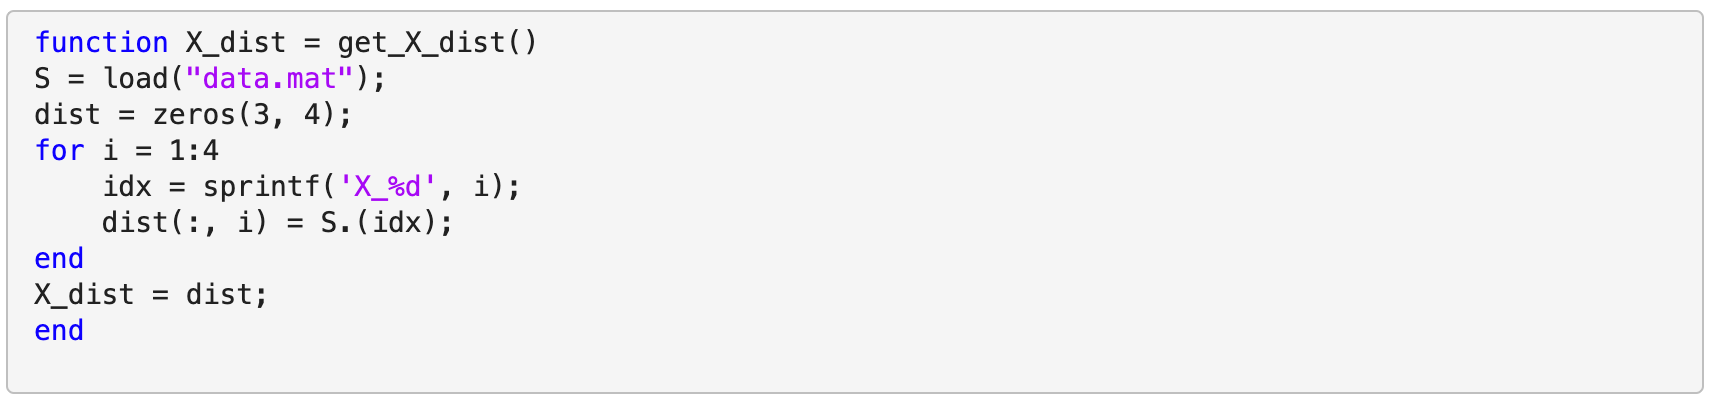
\includegraphics[width=0.9\linewidth]{X_dist}
		\caption{$\bb{T}_4$ generator}
		\label{fig:t4}
	\end{figure}

	\begin{figure}
		\centering
		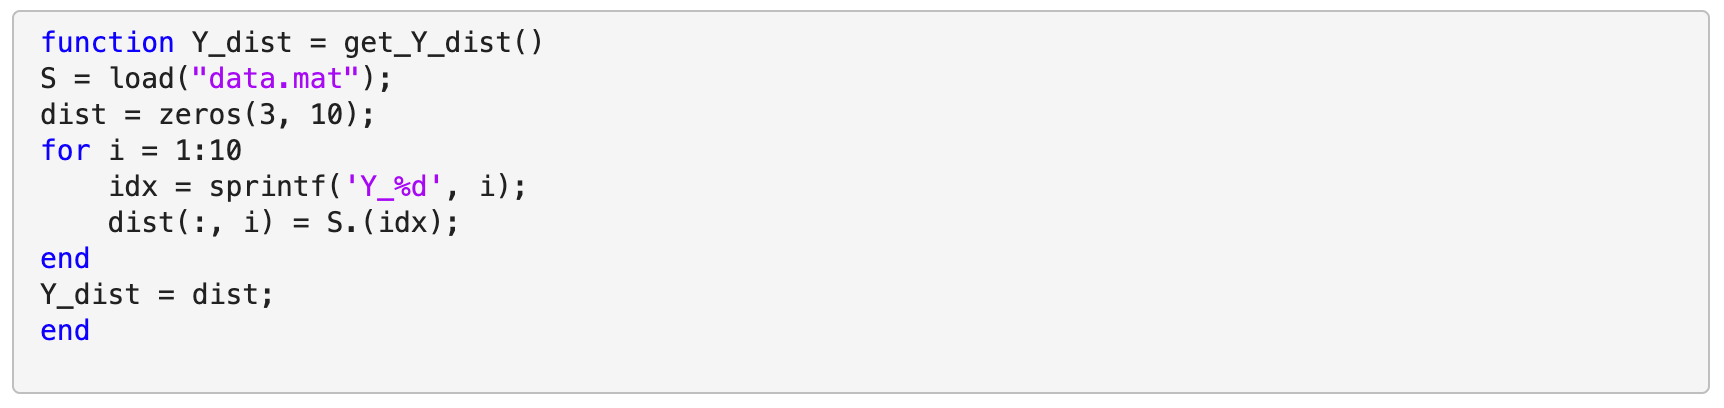
\includegraphics[width=0.9\linewidth]{Y_dist}
		\caption{$\bb{T}_{10}$ generator}
		\label{fig:t10}
	\end{figure}

	\begin{figure}
		\centering
		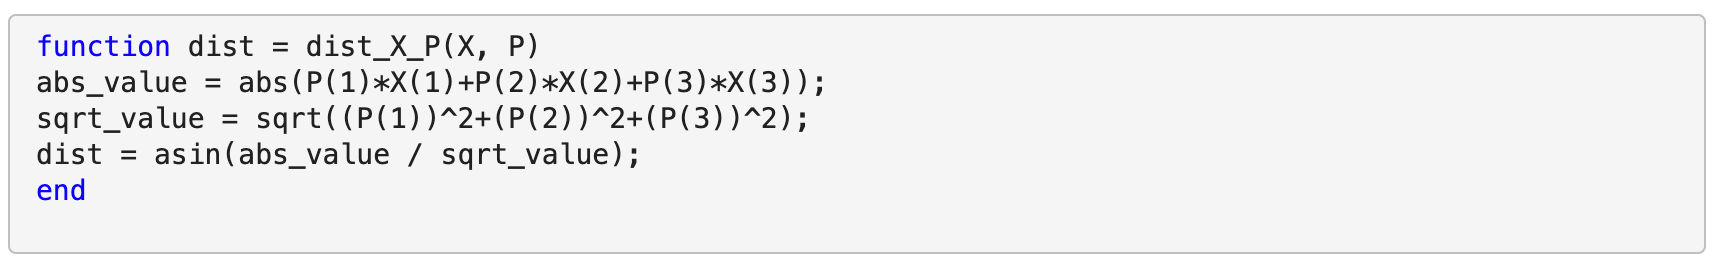
\includegraphics[width=0.9\linewidth]{dist_X_P}
		\caption{Distance function from point to G}
		\label{fig:dist}
	\end{figure}
	
	\begin{figure}
		\centering
		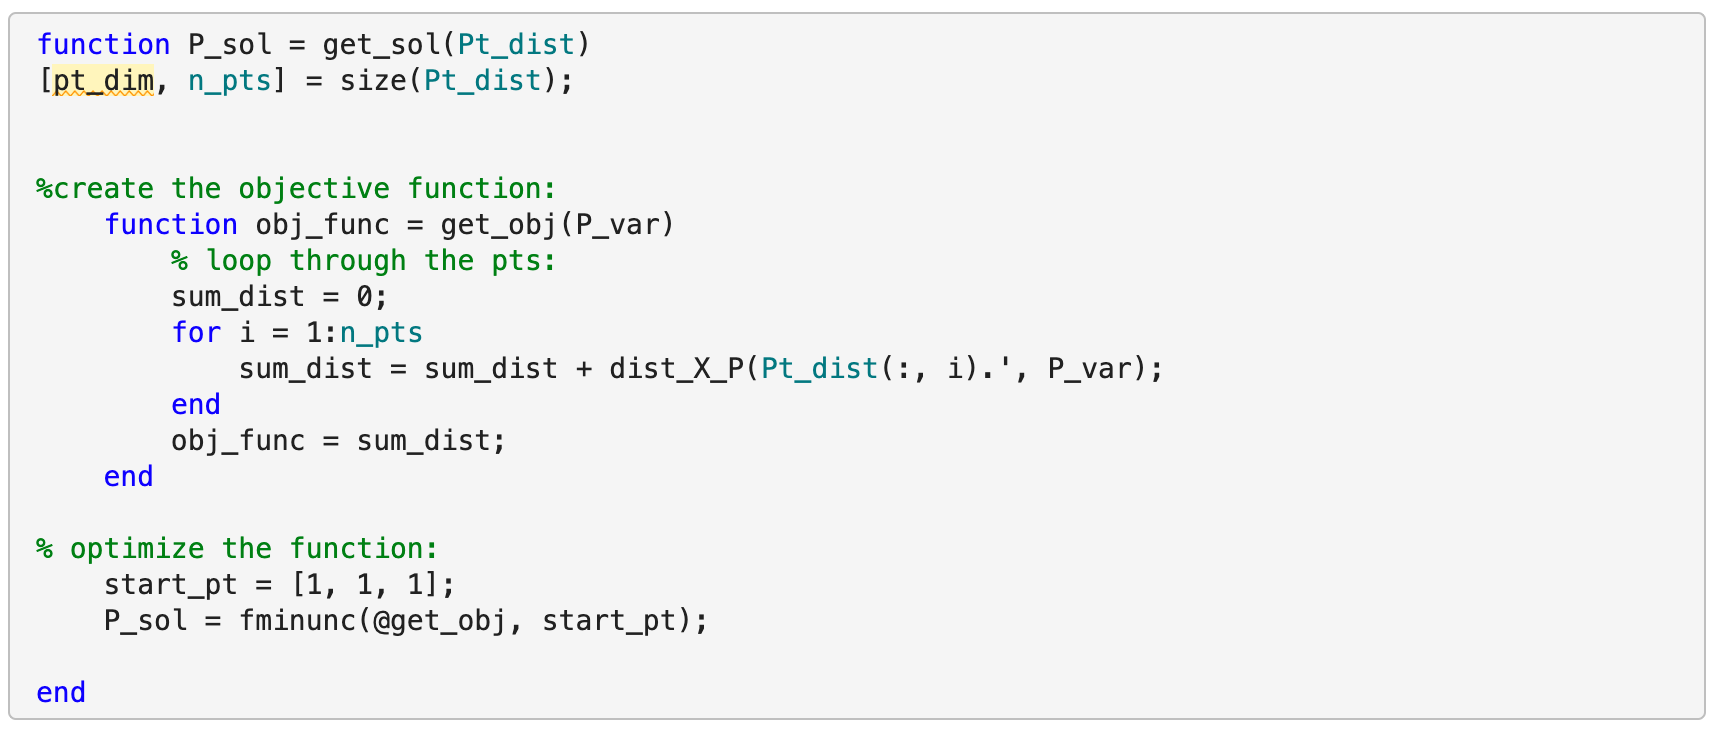
\includegraphics[width=0.9\linewidth]{get_sol}
		\caption{Solution function}
		\label{fig:sol}
	\end{figure}
	
	\begin{figure}
		\centering
		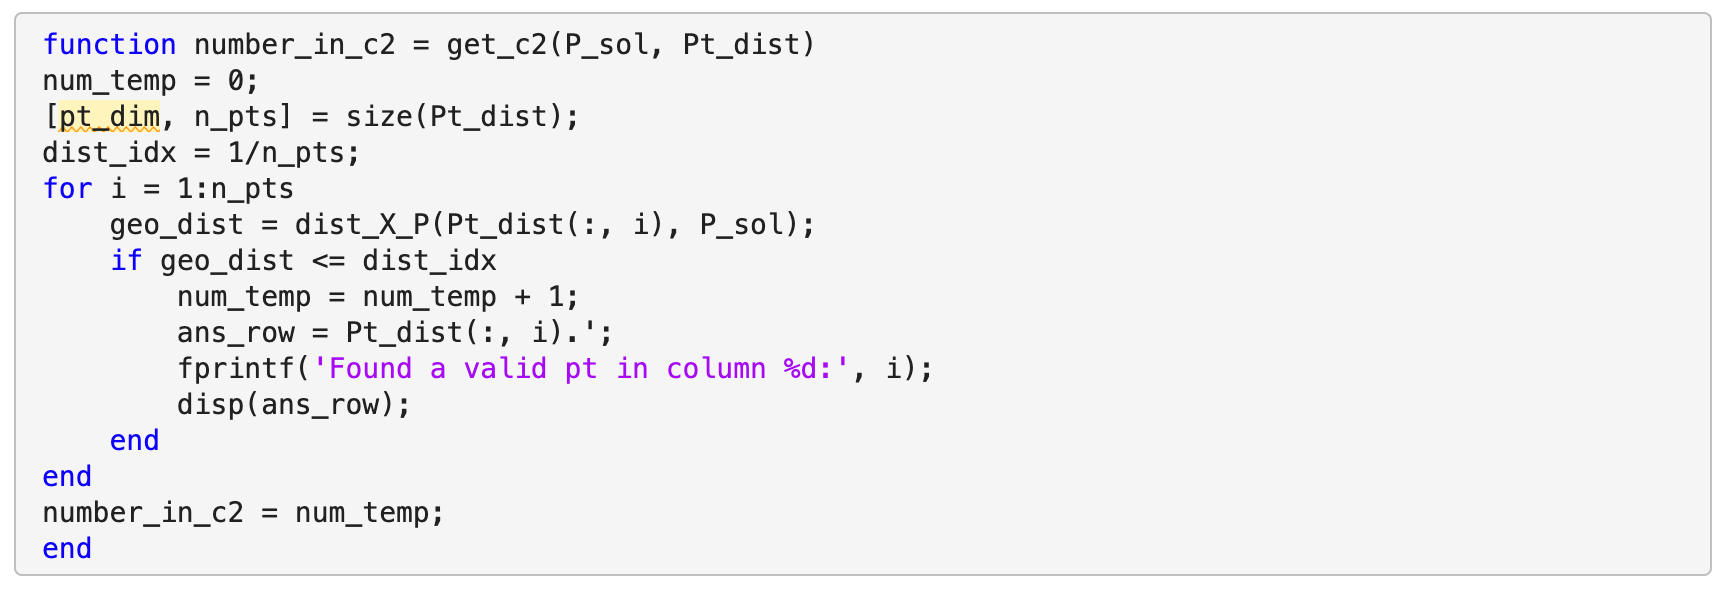
\includegraphics[width=0.9\linewidth]{get_c2}
		\caption{Final answer of clustered point}
		\label{fig:c2}
	\end{figure}
	\newpage
	
	\subsection{Calculation results analysis}
		\subsubsection{Results for $\bb{T}_2$}
		With no surprise, the optimal plane is $P_0: x=0$ with optimal variable [1, 0, 0] as shown in the figure \ref{fig:c3}. But one thing to notice is that our solution for $\bb{T}_2$ is only one of the infinite many solution. Theoretically, any great circle passes through the antipodal points could work. Since in any of these cases, the sum of geodesic distance of all the points in $\bb{T}_2$ to the great circle is 0 and thus make it an optimal solution. In such case, the number of clustered points around the great circle is 2. This is also the maximum number of clustered points we could get in such configuration with 
		\[ Max \{\#  \{ j:dist_{{\bb{S}}^2} (G, P_j)\leq \dfrac{1}{2} \}\} = n = 2\]
		A graphical result can be seen in the figure \ref{fig:g2} as below.
		In this graph, great circle C represents our optimal great circle corresponds to plane $P_0 : x = 0$. Another possible solution C2 is also shown in the graph, which corresponds to another optimal plane $P_2: y = 0$. \par 
		Click this link if you want to see the whole graph for $\bb{T}_2$ yourself and play with it. \par 
		\url{https://www.geogebra.org/calculator/yry46acv}
		
		\begin{figure}[b]
			\centering
			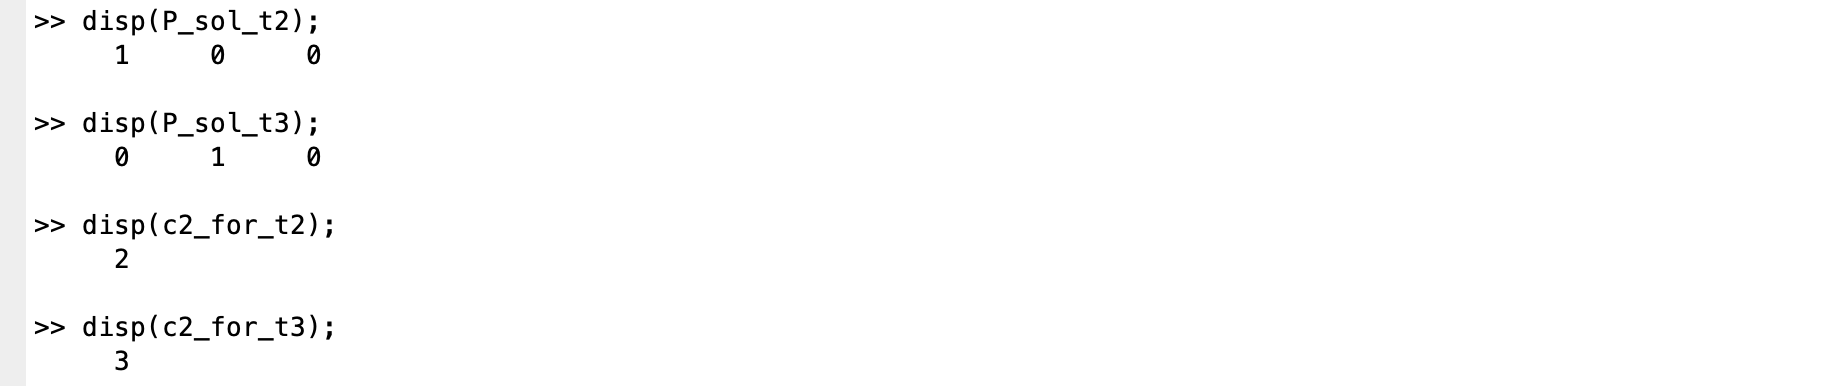
\includegraphics[width=0.9\linewidth]{t2_t3}
			\caption{Results for $\bb{T}_2$ and $\bb{T}_3$}
			\label{fig:c3}
		\end{figure}

		\begin{figure}
			\centering
			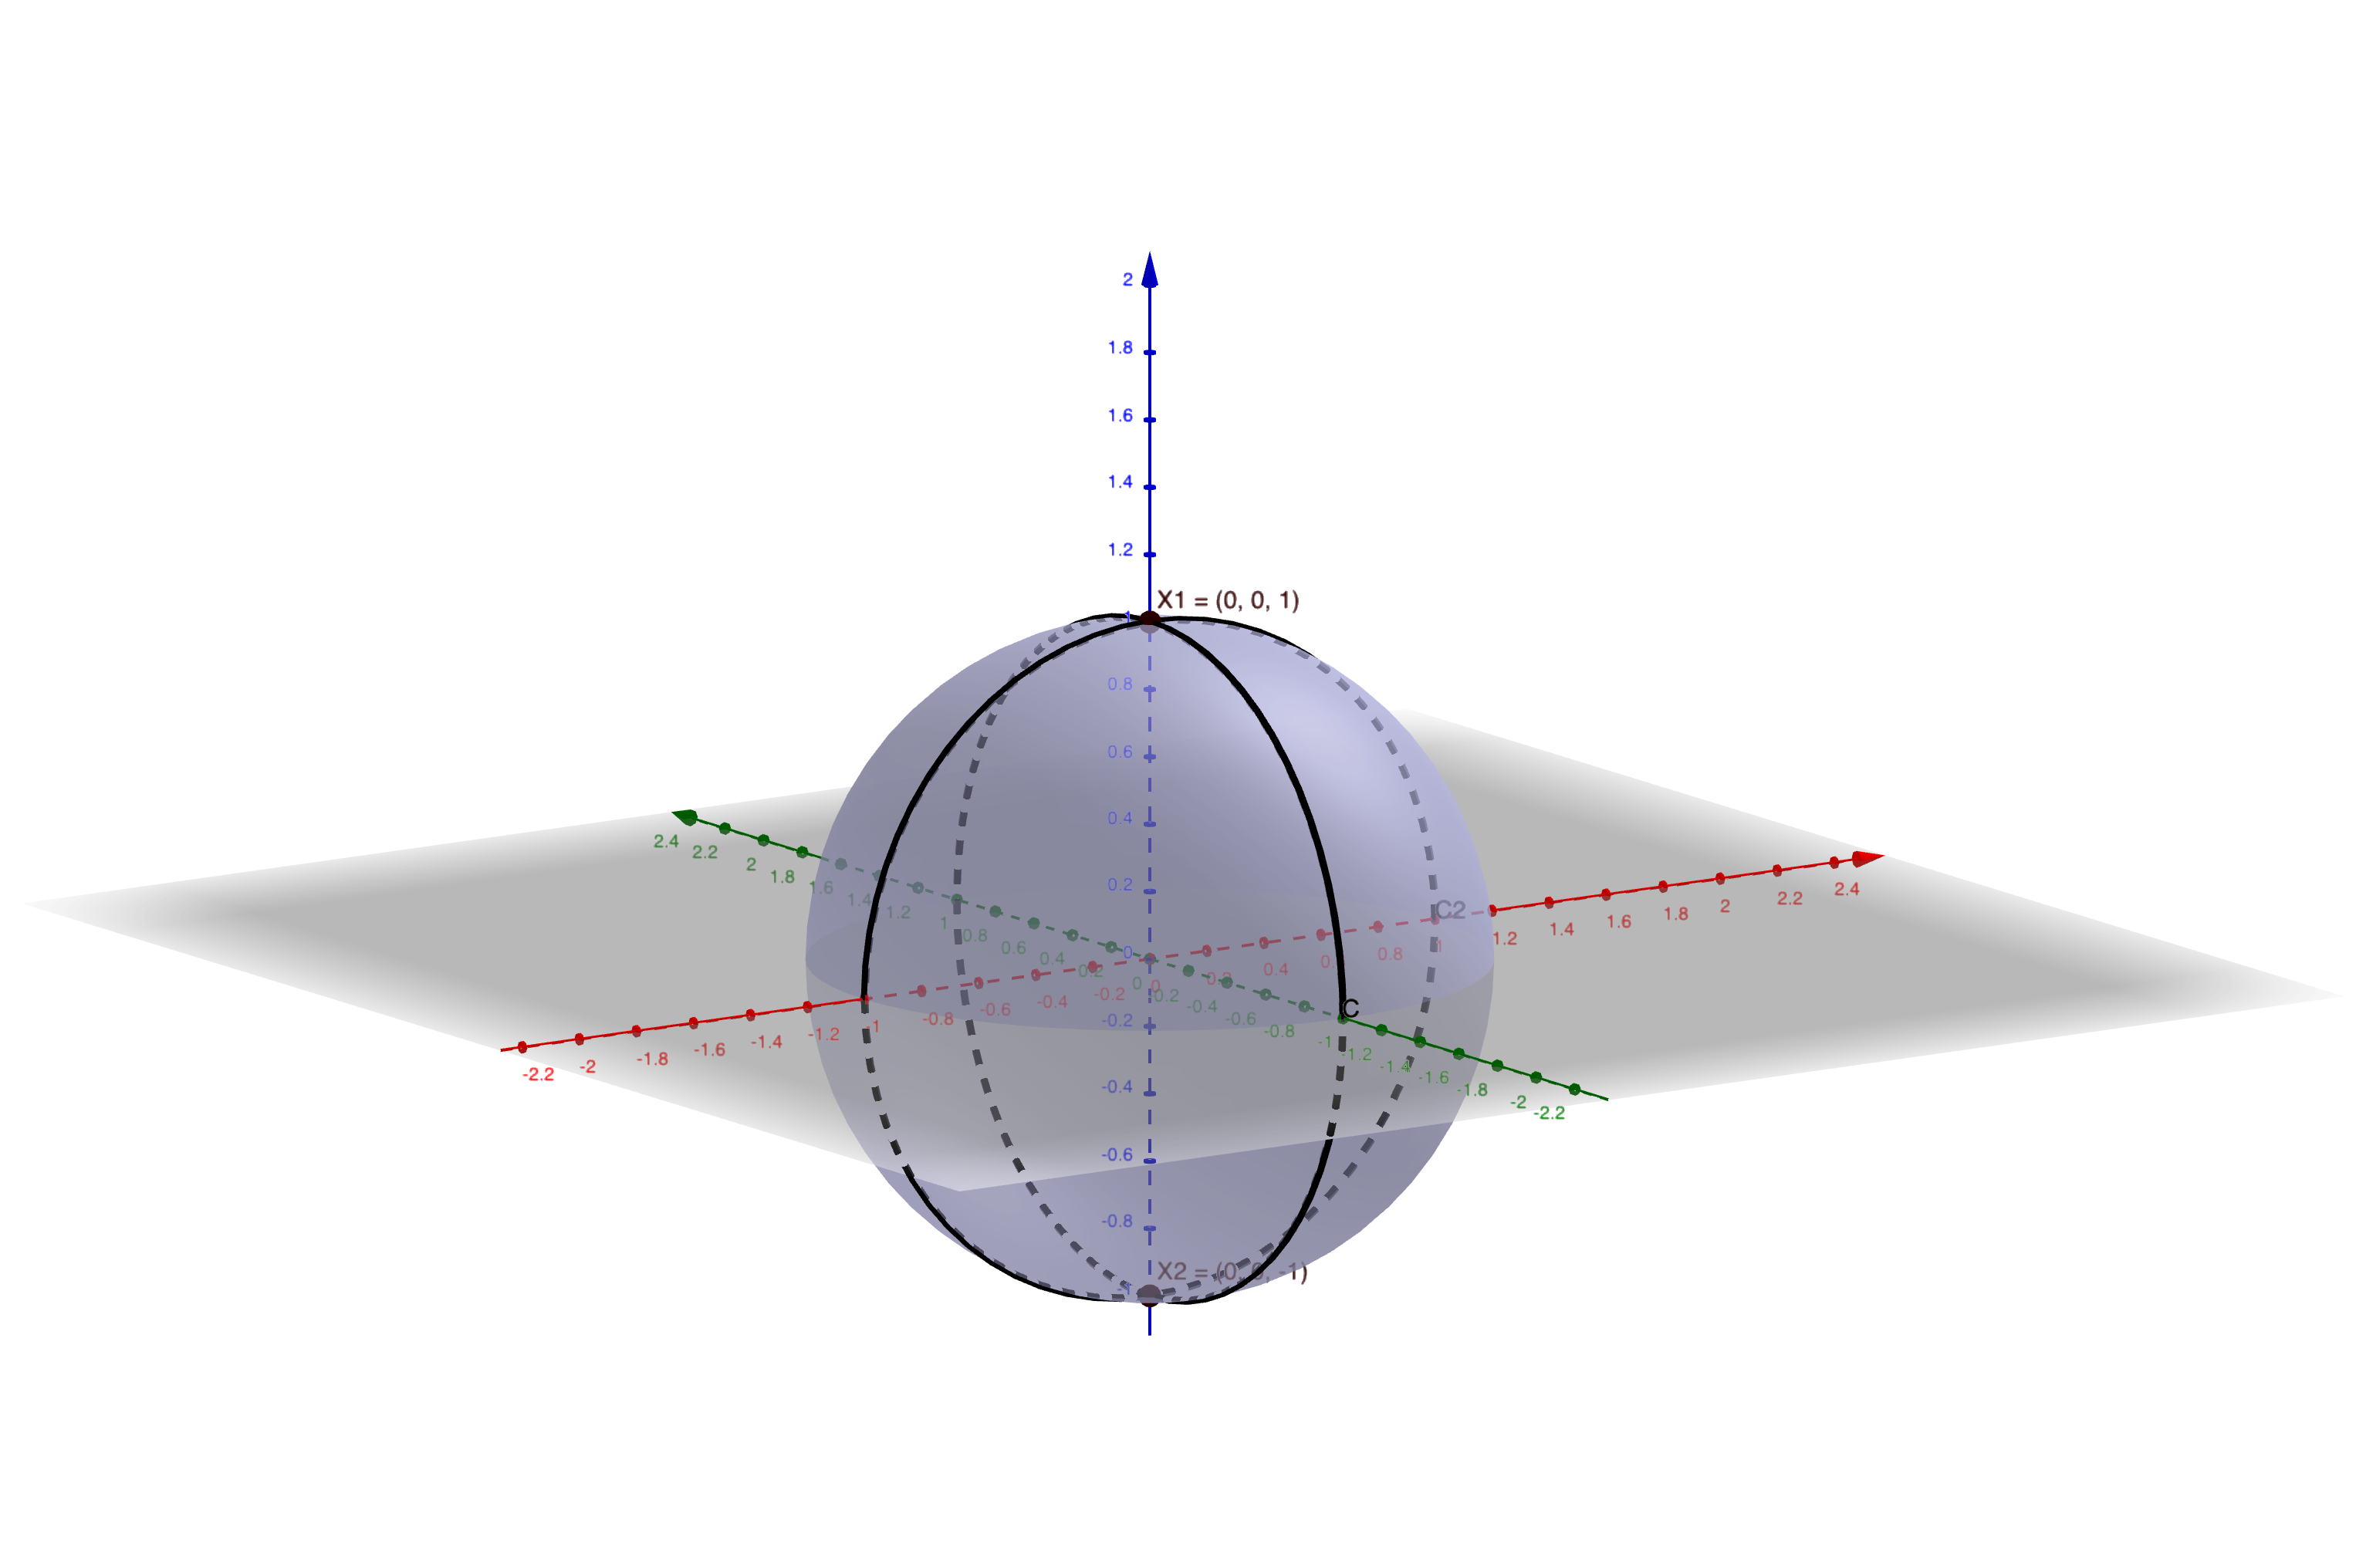
\includegraphics[width=1.1\linewidth]{T2}
			\caption{Graphical results for $\bb{T}_2$ }
			\label{fig:g2}
		\end{figure}
		
		\subsubsection{Results for $\bb{T}_3$}
			The solution for $\bb{T}_3$ is also not a surprise since all the 3 points are in the same plane. The calculation told us: the optimal plane in this case is $P_0: y=0$ with optimal variable [0, 1, 0]. this result also conform with our visualization since when 3 points lie in the great circle, then the sum of geodesic distance of all the points in $\bb{T}_3$ to the great circle is also 0 and reaches the optimal solution. Same as before in $\bb{T}_2$, this is the maximum number of clustered points we could possibly get. In this case:
			\[ Max \{\#  \{ j:dist_{{\bb{S}}^2} (G, P_j)\leq \dfrac{1}{3} \}\} = n = 3\]
			But there is one difference between the results of $\bb{T}_2$ and the results of $\bb{T}_3$. it should not exist infinitely many optimal solutions for $\bb{T}_3$ whereas $\bb{T}_2$ has infinitely solutions. the calculation results also support our arguments. As we change the different starting points of the gradient descent algorithm, the optimal solution for $\bb{T}_2$ varies while the solution stays the same for $\bb{T}_3$ case as we change to the different starting points.\par 
			A graphical results could be found in the figure \ref{fig:g3} with the optimal great circle C passing through all the points in $\bb{T}_3$. \par 
			The link for this graph is: 
			\url{https://www.geogebra.org/calculator/z3peebt5}
			
			
		\begin{figure}
			\centering
			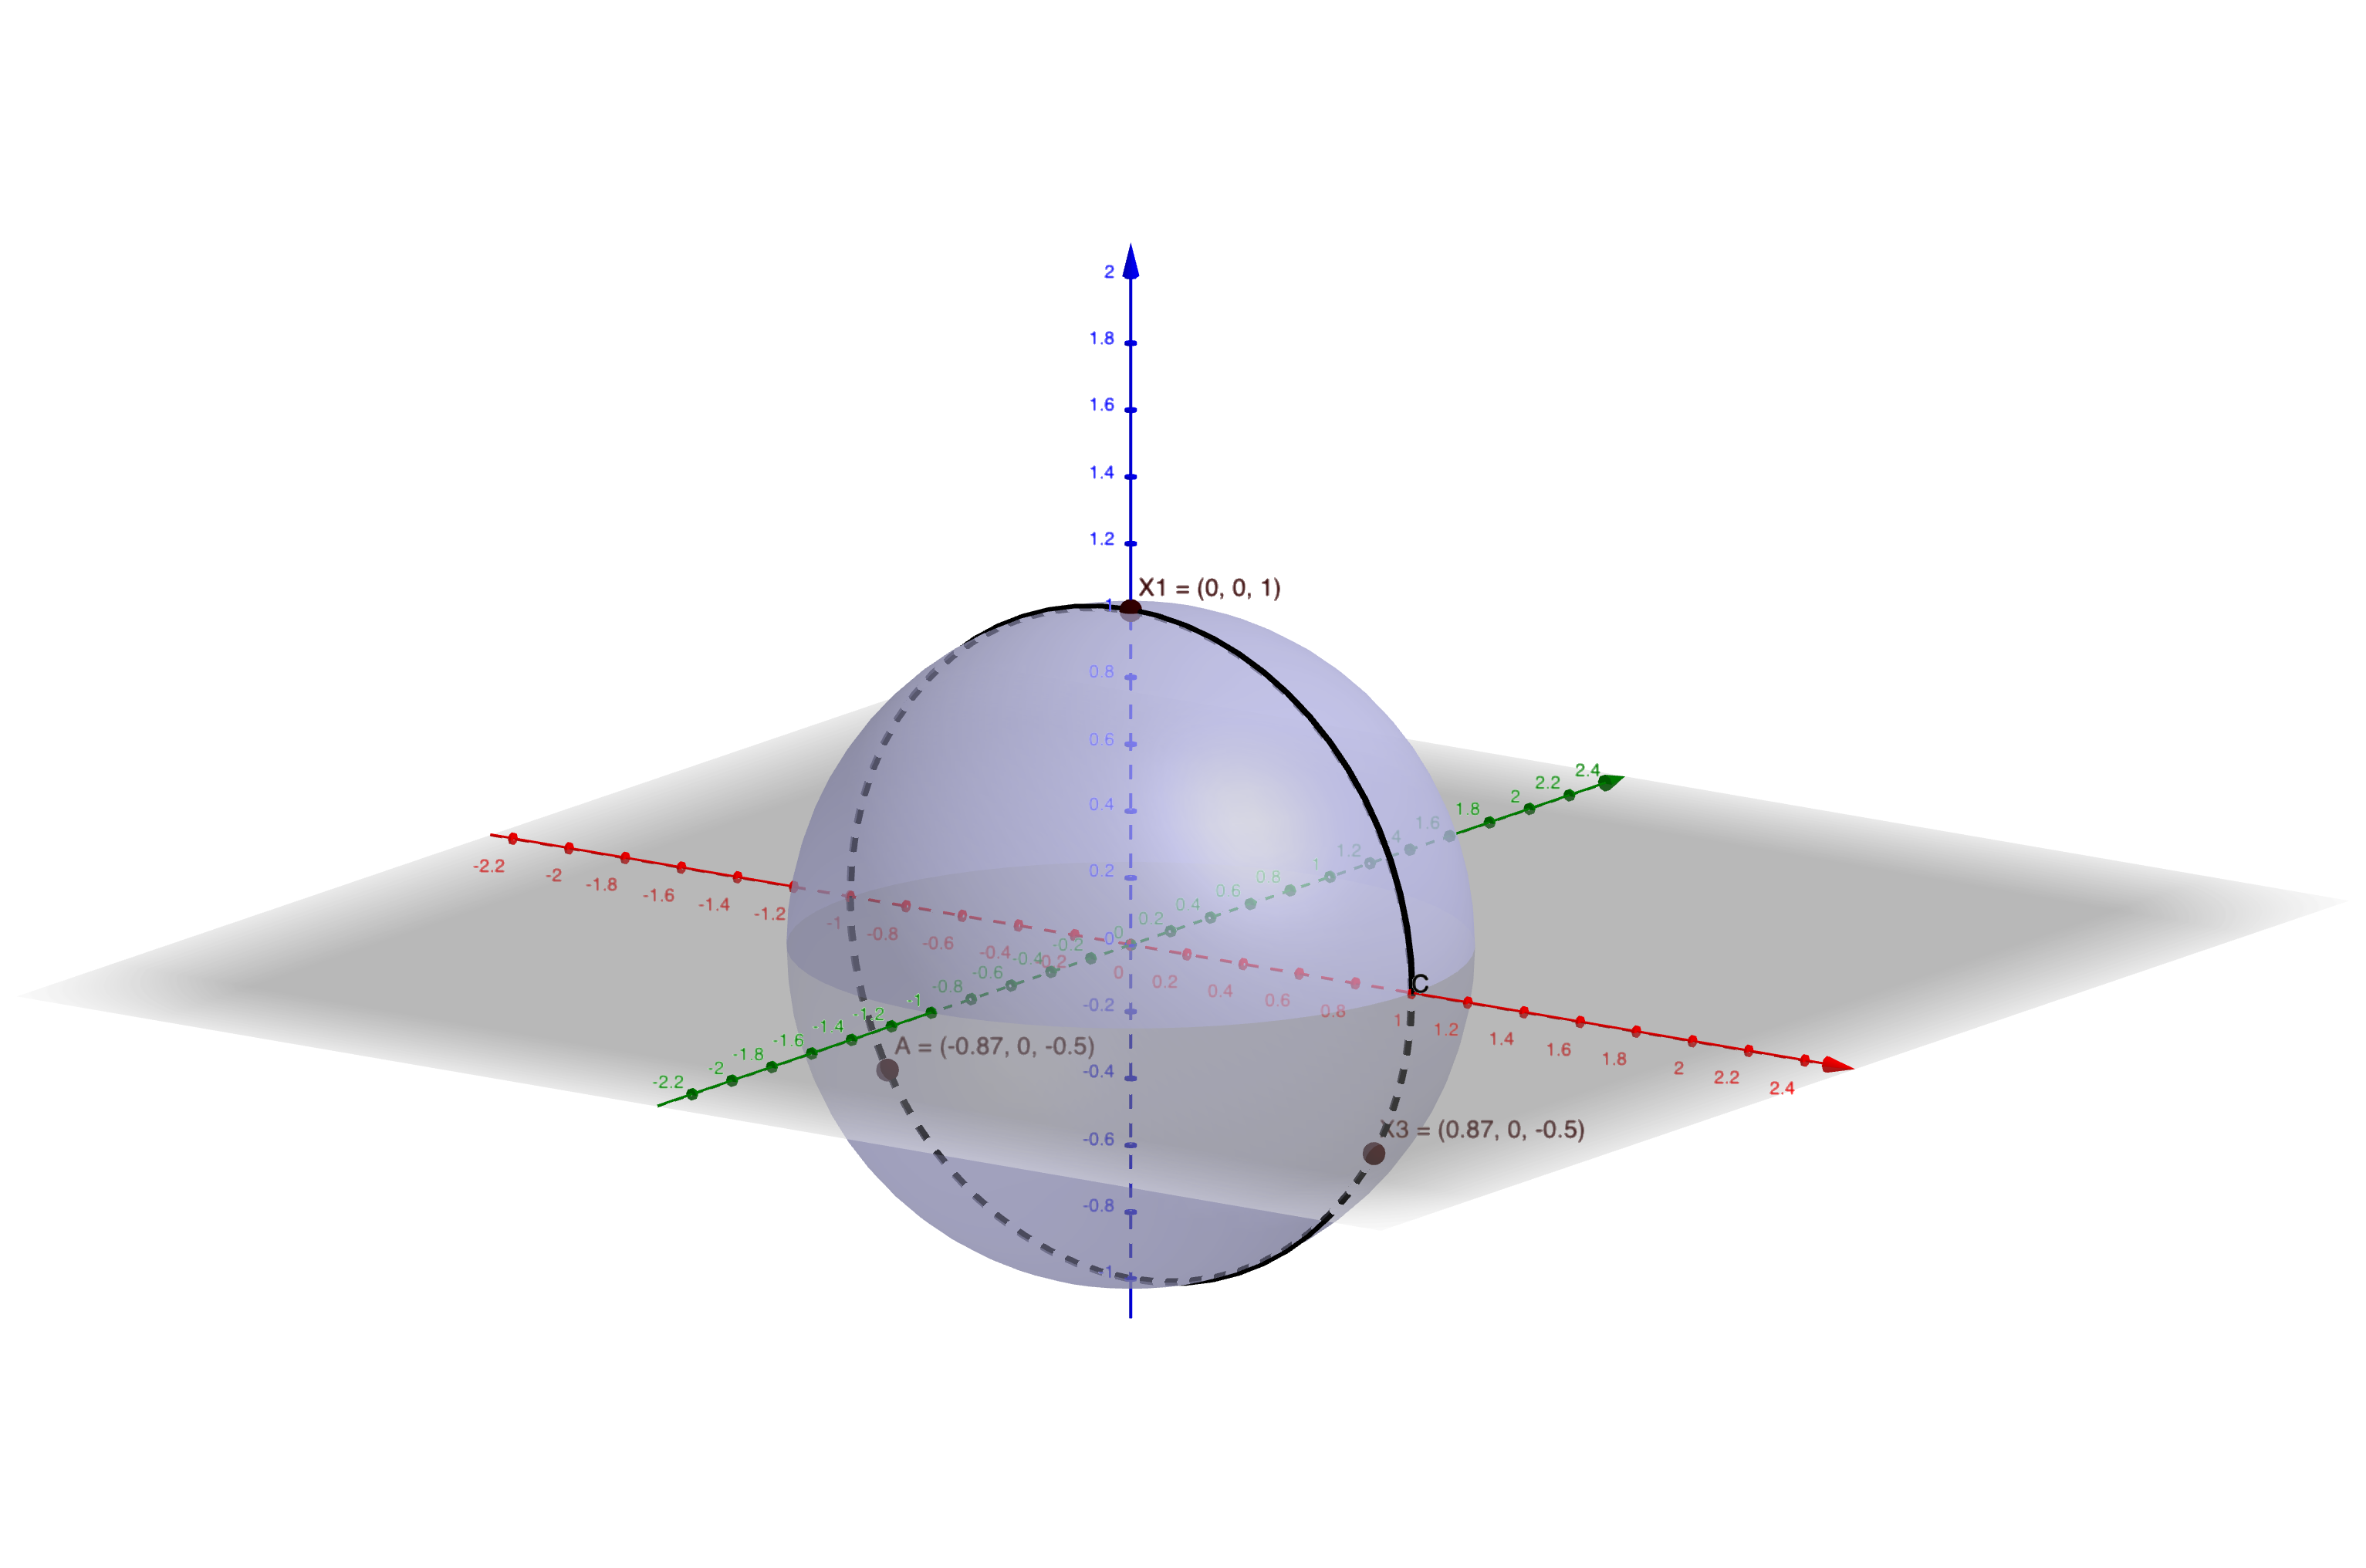
\includegraphics[width=1.1\linewidth]{T3}
			\caption{Graphical results for $\bb{T}_3$ }
			\label{fig:g3}
		\end{figure}
		
		\subsubsection{Results for $\bb{T}_4$}
			The story starts to become complicated for the case of $\bb{T}_4$, there is simply no guessable answer here since not all 4 points in the distribution are in the same plane. The optimal answer we got from the command line could be found in figure \ref{fig:c4}. And the graphical results could be found in figure \ref{fig:g4}.\par 
			As usual, you could access this graph by clicking the link: \url{https://www.geogebra.org/calculator/d9puknkh} \par 
			In figure \ref{fig:c4}, we could see that the optimal plane for the point distribution is $P_o = [1.1491, 0.9496, 0.9013]$ with corresponding plane equation: $1.1491x+0.9496y+0.9013z=0$. This is also the plane where the optimal great circle C lies in the figure \ref{fig:g4}. As we compare our optimal distance (The distance from each points to optimal great circle) to $\frac{1}{n} = \frac{1}{4}$, only two points are valid to be categorized into clustered points. These two points are: $(0, \dfrac{\sqrt{3}}{2}, 	-\dfrac{1}{2}) , (\dfrac{3}{4}, -\dfrac{\sqrt{3}}{4}, -\dfrac{1}{2})$ which has been highlighted in figure \ref{fig:g4} using red colour.\par 
			Overall, in this case with n = 4:
			
			\[ Max \{\#  \{ j:dist_{{\bb{S}}^2} (G, P_j)\leq \dfrac{1}{4} \}\} = 2\]
			But do notice that our calculation is based on the gradient descent algorithm. The existence of another optimal solution is possible by varying the starting points. As mentioned before, we have attempted many different starting points with the same settings. Although we always get the same optimal results in our experiments, it does not represent that we have found the global optimal solution. But this is at least a repetitive local optimal solution, it could help us to get some sense of the optimal configuration we are after. 
			With some close observation of the figure \ref{fig:g4}, we could find that only one point ($x_2$) is on the optimal great circle C.
			
		
		\begin{figure}
			\centering
			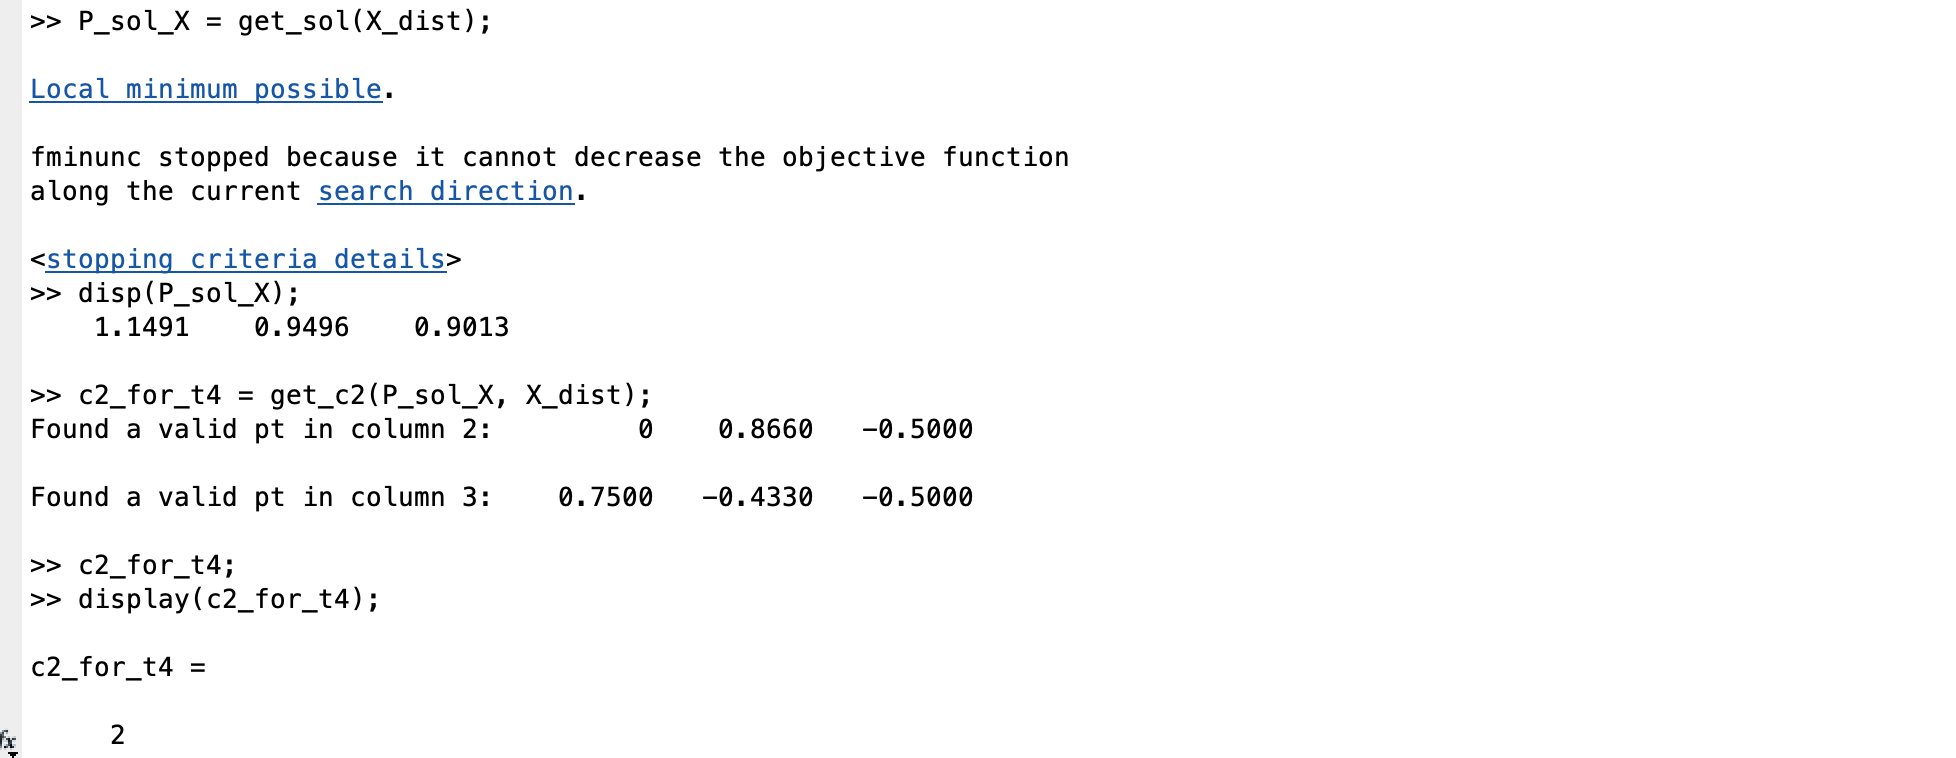
\includegraphics[width=1.1\linewidth]{t4_line}
			\caption{command line output results for $\bb{T}_4$ }
			\label{fig:c4}
		\end{figure}
		
		\begin{figure}
			\centering
			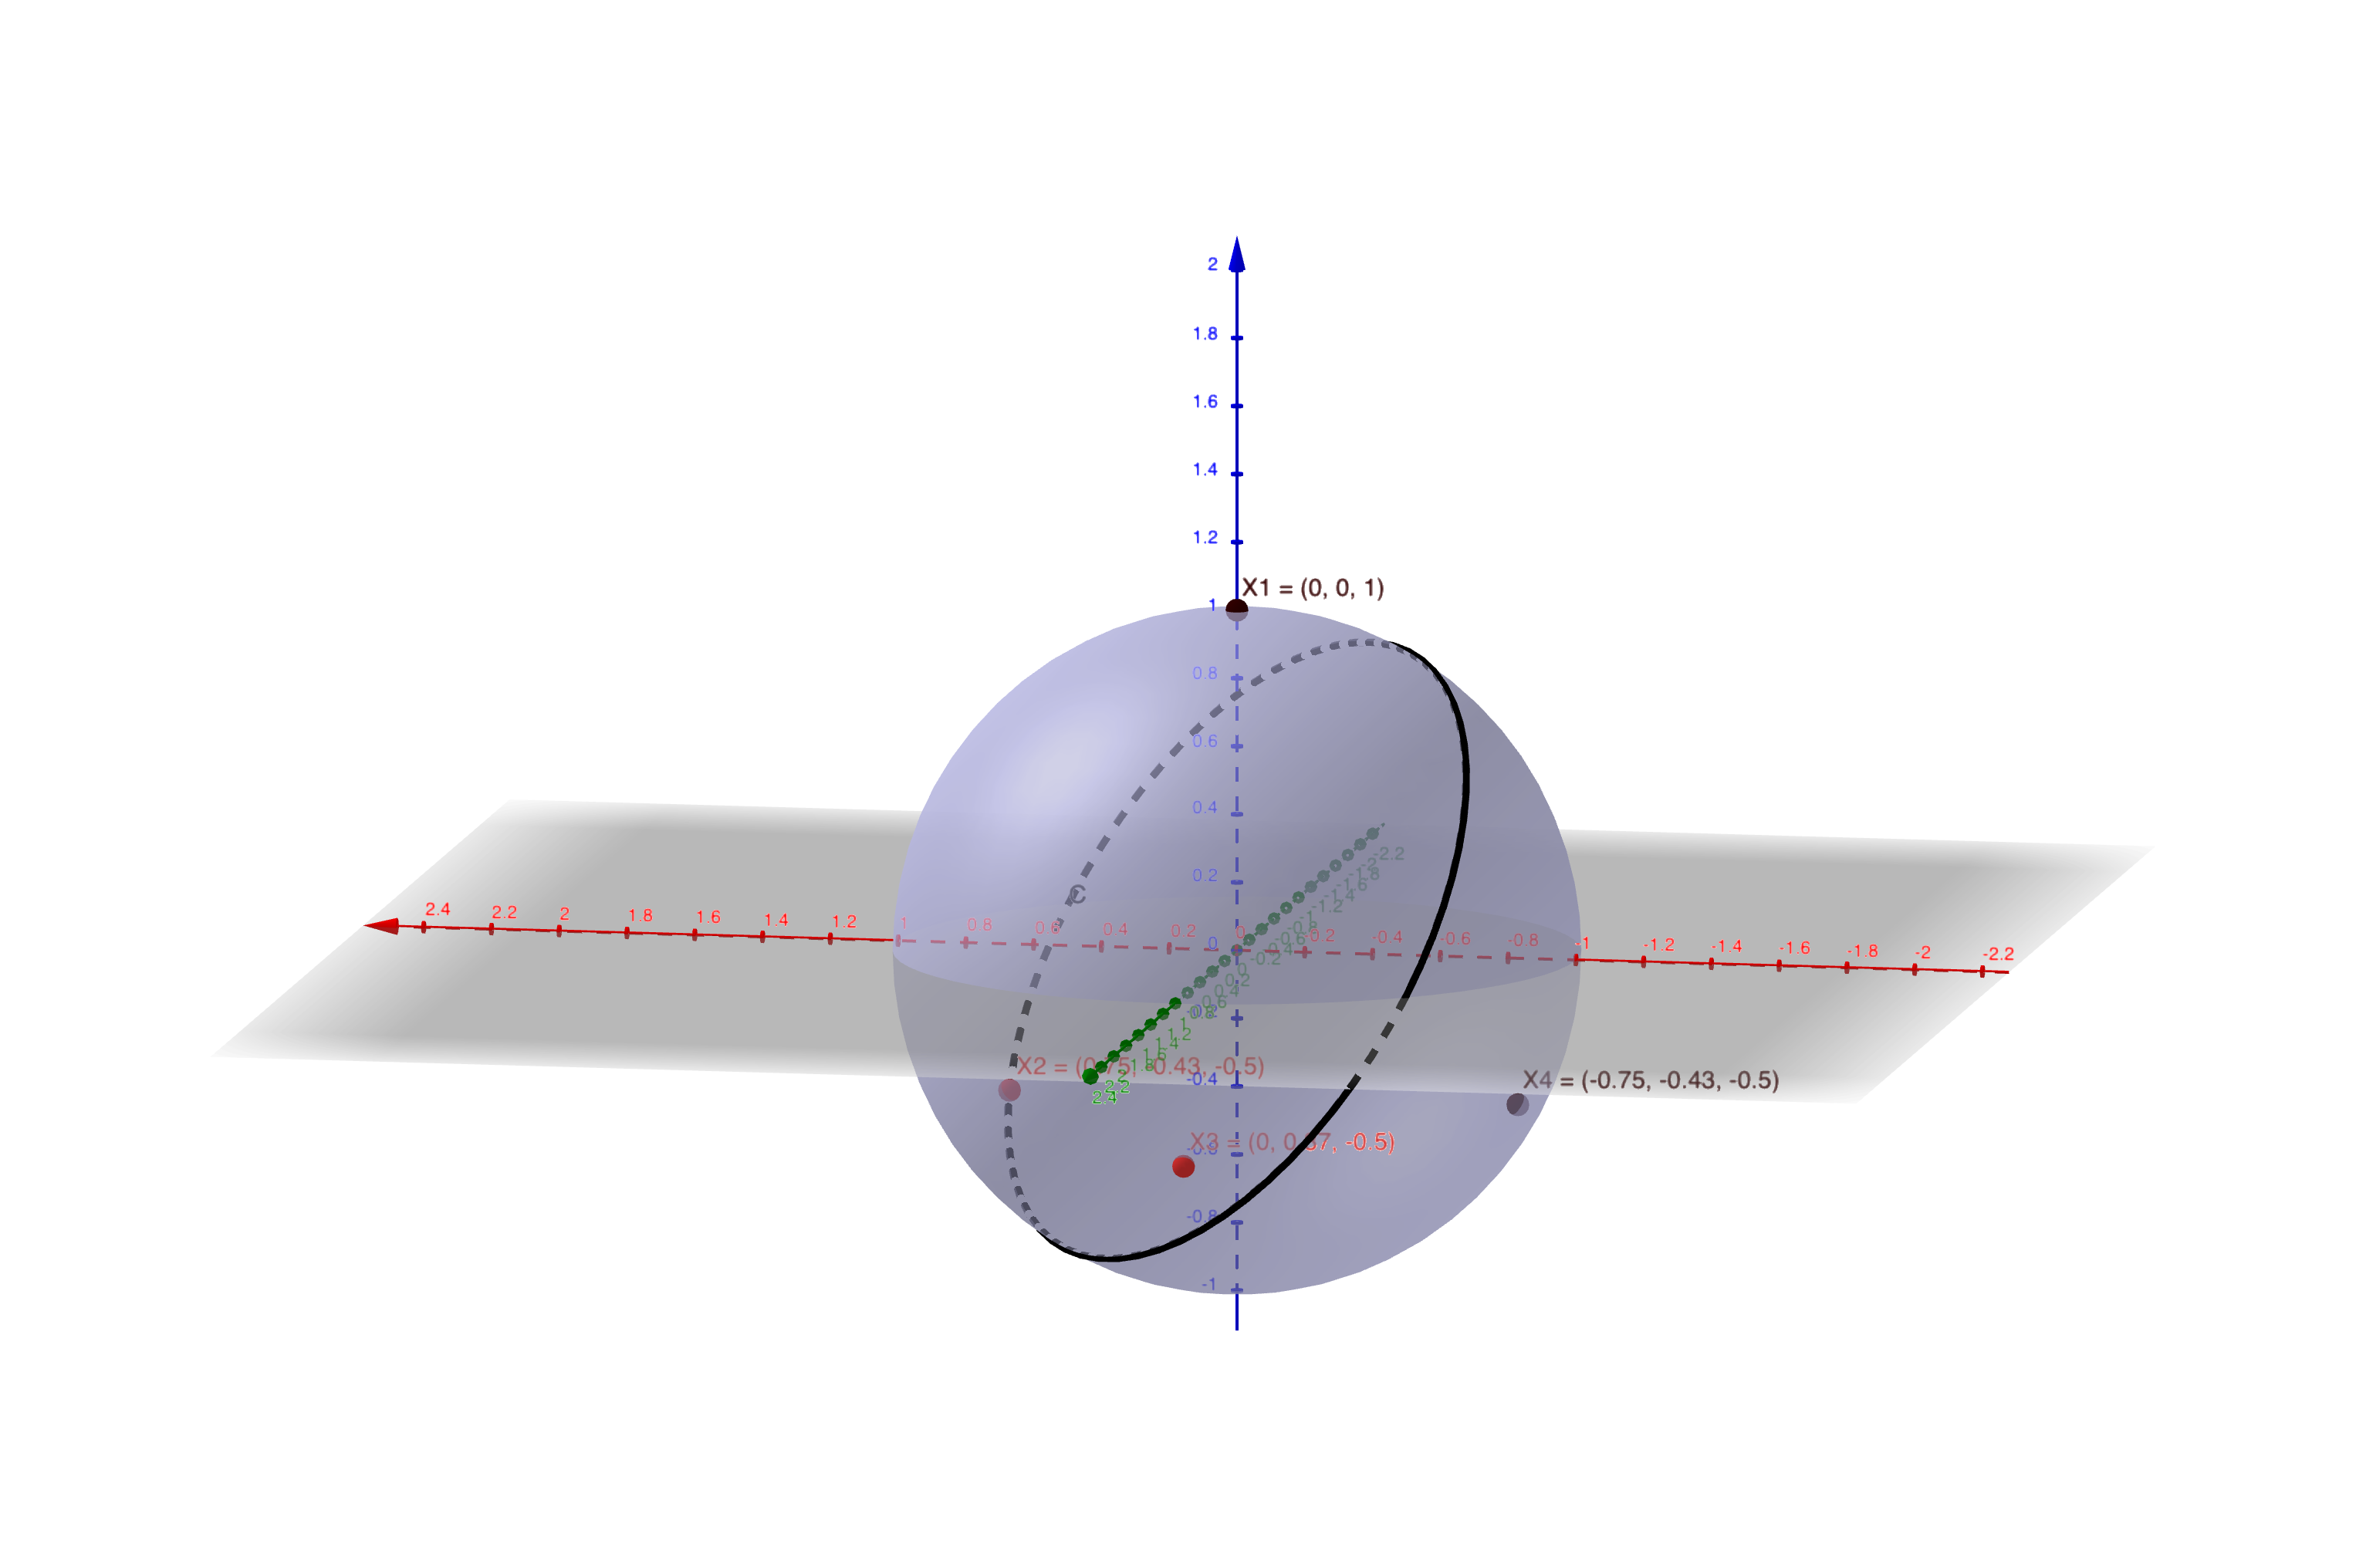
\includegraphics[width=1.1\linewidth]{T4}
			\caption{Graphical results for $\bb{T}_4$ }
			\label{fig:g4}
		\end{figure}

		\subsubsection{Results for $\bb{T}_{10}$}
			As we mentioned in the previous section, the coordinates of all the points in $\bb{T}_{10}$ are extremely hard to get. However, thanks to the results from this paper \cite{sugimoto_2015_exact}, we are able to run our algorithm. And the result we get is pretty interesting as shown in the figure \ref{fig:c10} and figure \ref{fig:g10}. \par
			As usual, you could gain the access for this graph at : \url{https://www.geogebra.org/calculator/n4yatawk}\par
			
			First of all, we have to emphasis this is not said to be the global optimal solution, rather than a repetitive local minimum which could give us a sense of intuition like above.\par
			From figure \ref{fig:c10}, the results give us the optimal plane $P_o = [0.6830, 1.2316, 1.5448]$ with corresponding plane equation: $P_o: 0.6830x+1.2316y+1.5448z=0$. The optimal great circle C is illustrated in the figure \ref{fig:g10}. Same as the case in $\bb{T}_4$, the optimal great circle C only passes through 1 point ($x_3$) in the distribution. one surprising result is that the final clustered points is still 2 (marked with red in figure \ref{fig:g10}) even though it has 10 points now. based on some observation on figure \ref{fig:g10}, it's not too hard to find:
			\begin{enumerate}
				\item $\bb{T}_{10}$ seems to have some sort of symmetry around the z-axis in this graph. and such symmetry scatters the points to be far enough within the bandwidth around one great circle.
				\item As n increases, the bandwidth $\frac{2}{n}$ around the great circle decreases. It's harder for points to be in the bandwidth if they are distributed evenly.
			\end{enumerate} 
		
			Overall, in this case with n = 10:
			
			\[ Max \{\#  \{ j:dist_{{\bb{S}}^2} (G, P_j)\leq \dfrac{1}{10} \}\} = 2\] 
		
		\begin{figure}
			\centering
			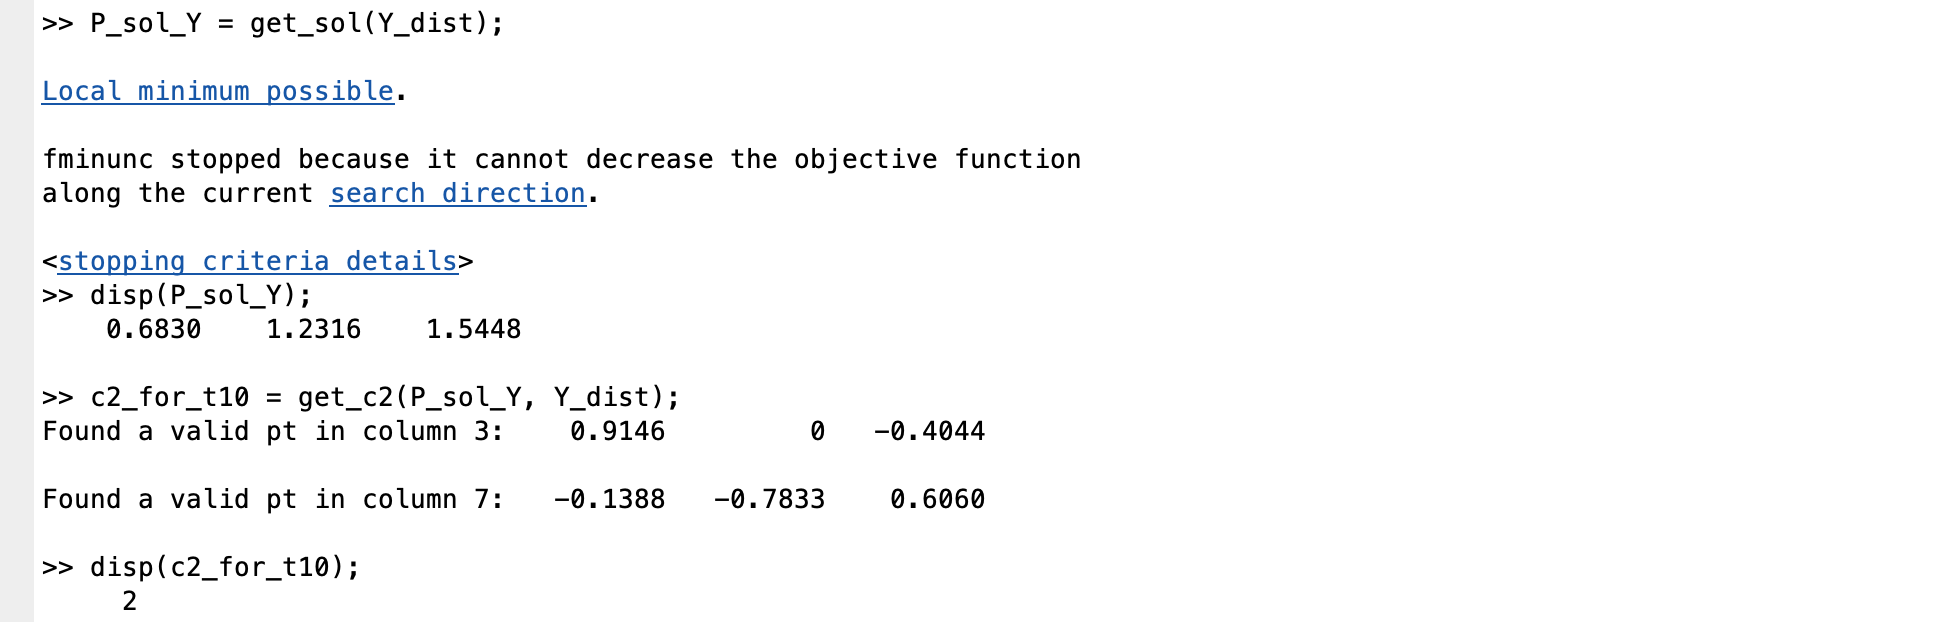
\includegraphics[width=1.1\linewidth]{t10_line}
			\caption{command line output results for $\bb{T}_{10}$ }
			\label{fig:c10}
		\end{figure}
		
		\begin{figure}
			\centering
			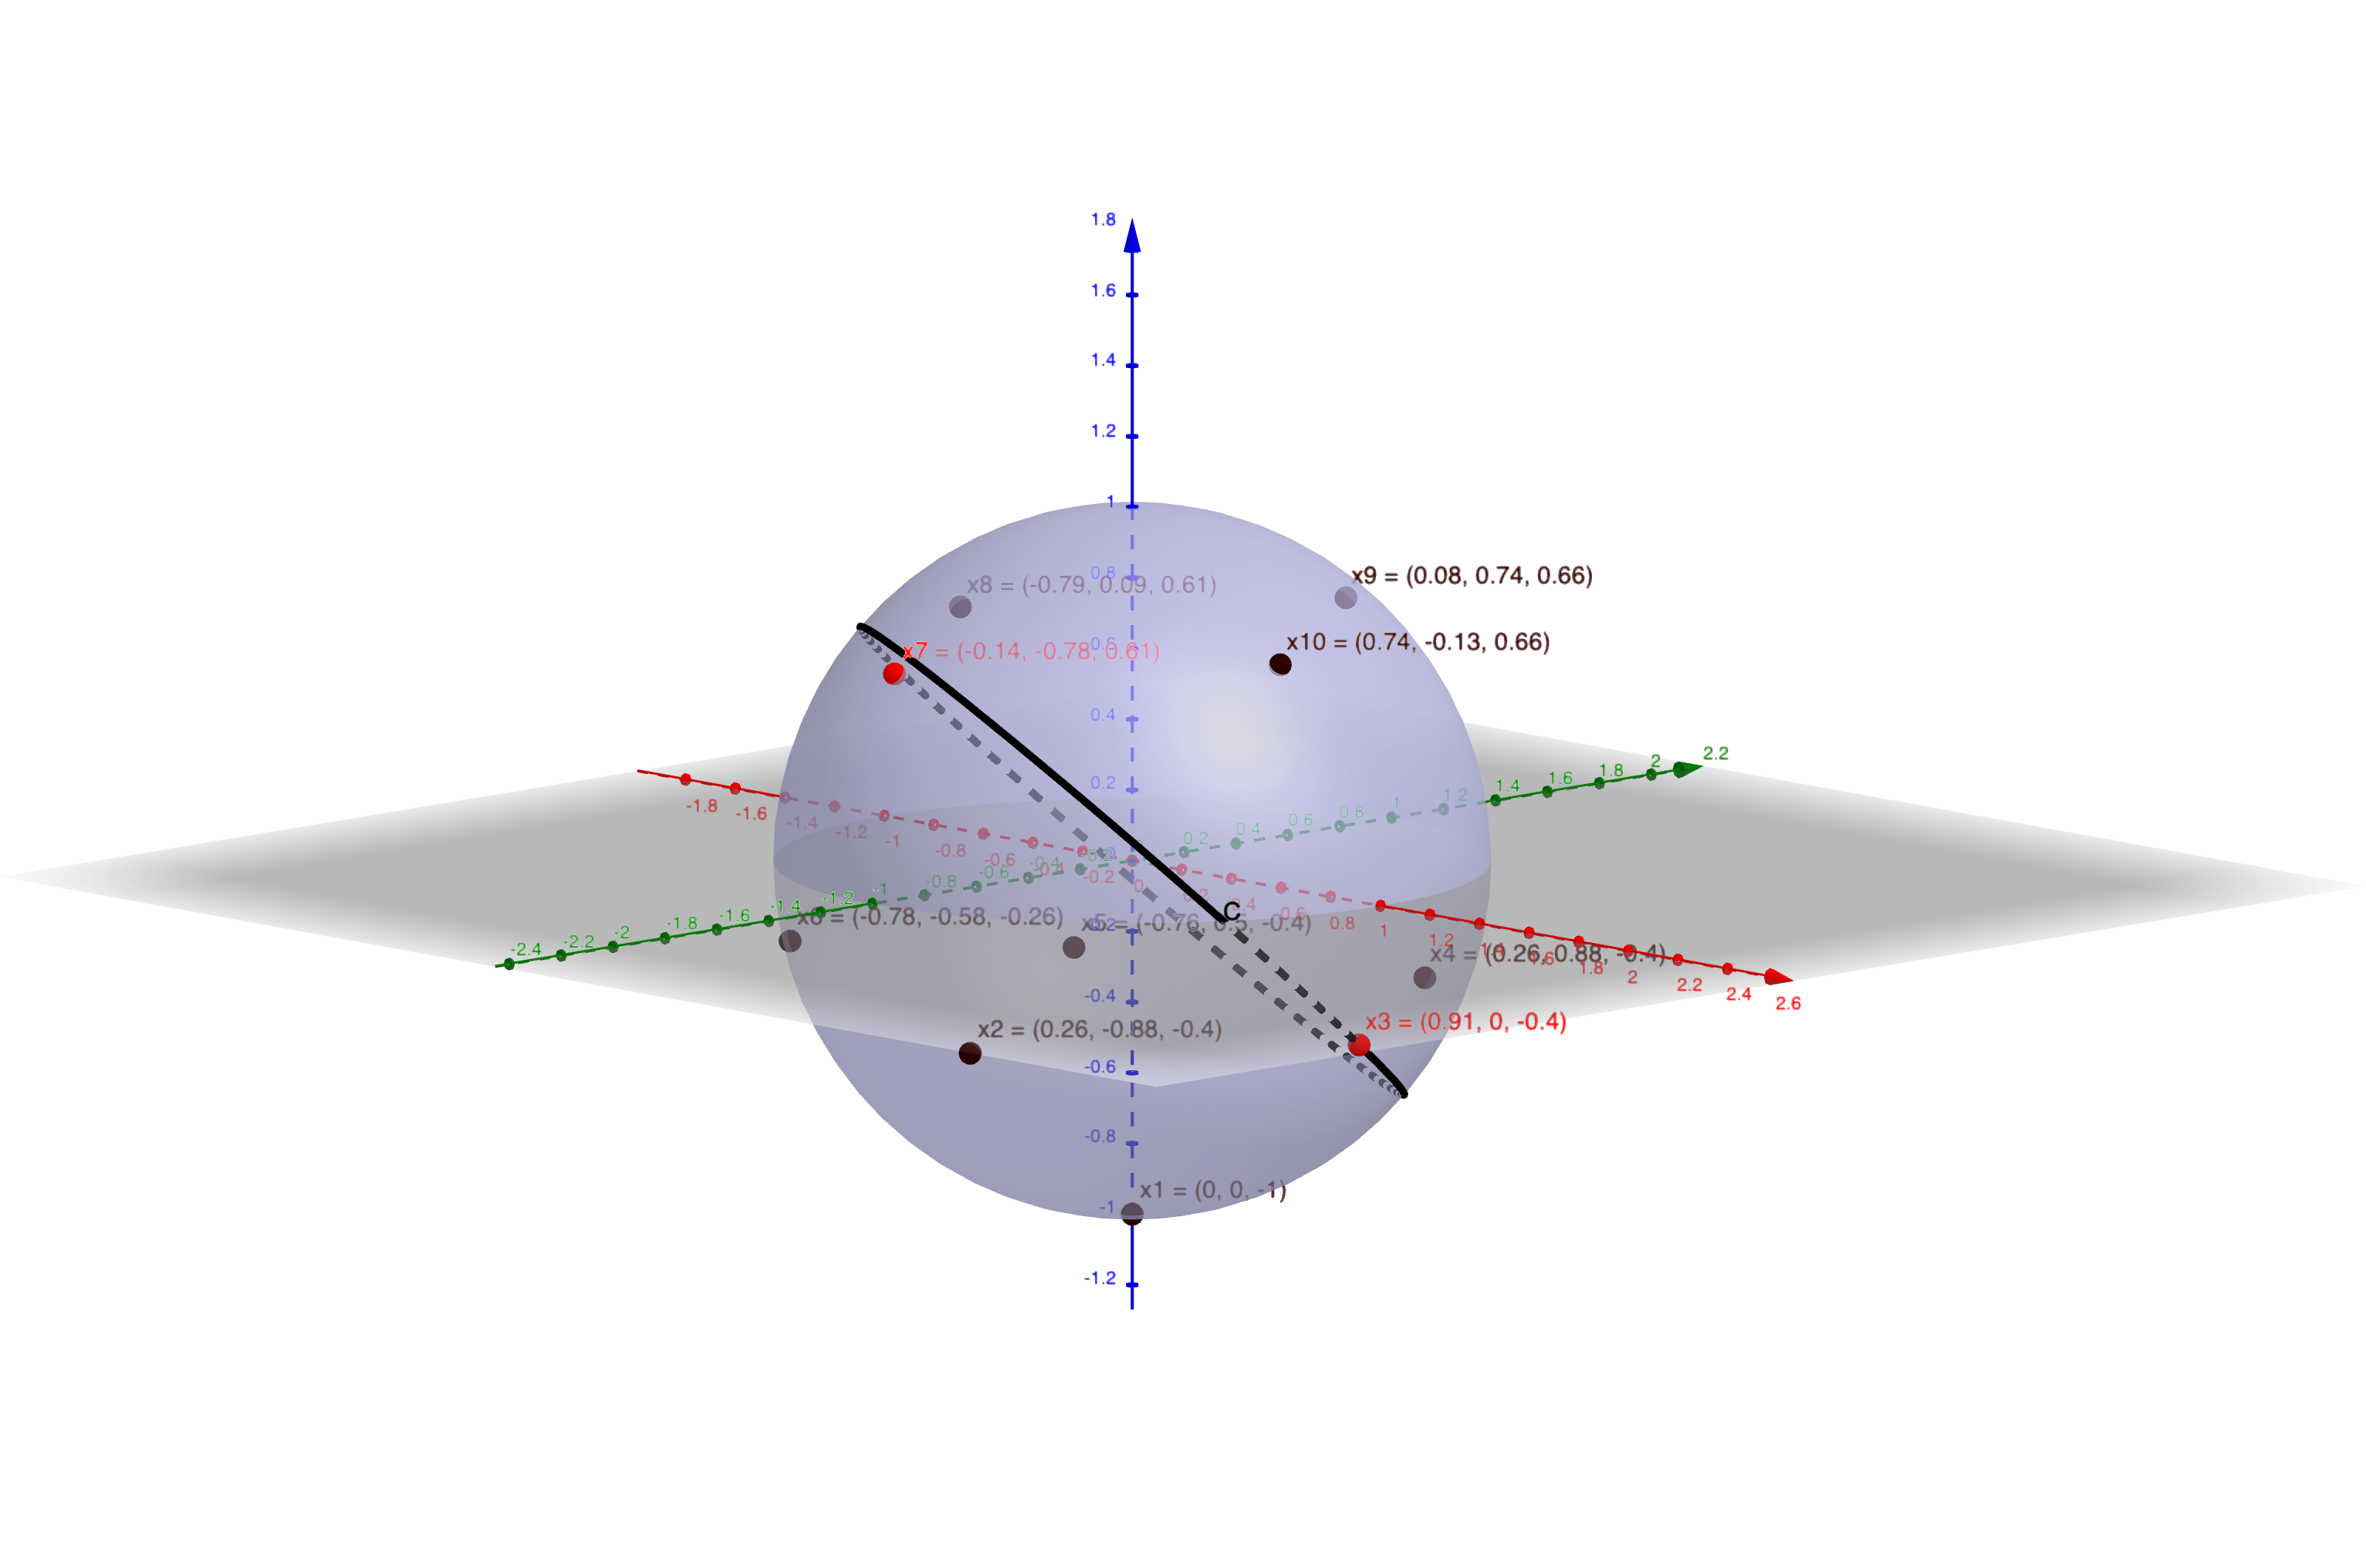
\includegraphics[width=1.1\linewidth]{T10}
			\caption{Graphical results for $\bb{T}_{10}$ }
			\label{fig:g10}
		\end{figure}
		
		\subsubsection{Summery for the results}
			Based on the results we see so far in the last subsection, we still have nothing to say about the condition 2 since our goal is not to get $C_n$ for some specific n. We want to find a special $C >0 $ which is independent of n. It is impossible to test all the $\bb{T}_n$, not to say that the solution of Tammes problem remains a mystery as well. Thus we could only hope that some abstract common symetries can be found between different $\bb{T}_n$, and use such symmetry to generate $C>0$ that satisfies the condition 2.\\
			One thing we could say based on the above results is that $C \geq C_n \, \forall n \in \bb{N}$, thus we get : $C \geq 3$. \par
			One possible hypothesis is that: if $\bb{T}_n$ always contains some symmery $\forall n \in \bb{N}$ that makes points nearly evenly distributed in the sphere. As n increases, the bandwidth $\frac{2}{n}$ within any great circle G  could only contain a finitely many number of points and thus to proof the C is converge as n $\rightarrow \infty$.\par 
			However, this is a huge hypothesis, there are many mysteries in this claim we cannot solve at this time.\par
			Finally, here is a little summery table for all the final results: \par 
			\vspace{5mm}
			\begin{tabular}{|c|c|}
				\hline
				n & $C_n = Max \{\#  \{ j:dist_{{\bb{S}}^2} (G, P_j)\leq \dfrac{1}{n} \}\}$ \\
				\hline 
				2 & 2 \\
				\hline 
				3 & 3 \\
				\hline 
				4 & 2 \\
				\hline 
				10 & 2 \\
				\hline
			\end{tabular}
			
	\newpage
	\section{Condition 3: Equi-distribution/Evenly distributed}
		\begin{general}[c1]{Equi-distribution}
		For any positive integer n, there is a collection of points $\{ P_j^n \}_{j=1}^n$ such that 
		For any $f \in C^{\infty}(\bb{S}^2)$, \\
		$\lim\limits_{n \to \infty} \dfrac{1}{n} \sum_{j=1}^{n} f(P_j^n) = \dfrac{1}{4\pi} \int_{\bb{S}^2} f(P)dP$
		
		
		\end{general}
	
	
	This condition should have been the most difficult one to verify for me since it concerns the spherical harmonics and even coding theory. However, some paper have mentioned that Tammes' problem is actually one of the natural way to build equi-distributed point distribution.(see \cite{brauchart_2015_distributing}, 294) thus, the solution of any Tammes's problem naturally becomes a well-distributed point sets. This is an non obvious but no mystery result.\\
	More study regarding this subject is required.
	
	\vspace{10mm}
	\newpage
	\part{Evenly distributed point distribution construction}
	
	\newpage
	\section{Introduction to group-theoretic point distribution construction}
	In this last part of the report, we will use the point distribution construction method explained in \cite{lubotzky_1986_hecke} and discuss its possibility of satisfying those 3 conditions in part 2 of this report.
	In their paper \cite{lubotzky_1986_hecke}, they pose a new method to build a point distribution with the optimal uniformity in an efficient way. \par 
	Worth-noting that their `uniformity' has a high resemblance to the meaning of `evenly-distributed' in condition 3. \par
	They wish to make $\delta f$ as small as possible, where 
	\[ \delta f = \frac{1}{n} \sum^n_{j=1}f(x_j)-\int f \hspace{3mm} \]
	(From here onwards, we shall use $\bb{D}_n$ to denote the n-points distribution generated by group-theoretic construction method in \cite{lubotzky_1986_hecke}.)\par 
	However, in condition 3, we want to verify whether such $\delta f$ is asymptotically 0 as n $\rightarrow$ $\infty$. A detailed discussion will reserved for later sections.\par 
	Their idea of construction originates from the 3-D rotational group $SO(3)$. Instead of constructing each point individually, they form a countable subgroup $\Gamma \leq SO(3)$ and apply each rotational elements in the subgroup to one of the points on the sphere. Thus creating the whole distribution systematically. One benefit of such construction is rotation invariant. No matter what starting point you choose on the sphere, the resulting distribution will be identical with respected to sphere rotation. \par 
	As for the construction of such particular subgroup $\Gamma $, it should satisfy the condition mentioned in Theorem 1.5 in \cite{lubotzky_1986_hecke}.
	
	\newpage
	\section{$\bb{D}_n$ and Condition 1 }
	To verify condition 1, we need to show that for any positive integer n, there is a corresponding $\bb{D}_n$ such that for any $j,k = 1,..., n$ and $j\neq k$, \\
	dist$(x_j, x_k)$ $\geq \frac{c}{\sqrt{n}}$ \\
	for constance c and $x_j,x_k \in \bb{D}_n$.\par 
	To tackle this problem, we need to consider the following 2 steps:\\
	\begin{enumerate}
		\item we wish to find such distribution $\bb{D}_n$ for any n. But so far, we only know how to construct a subgroup $\Gamma$ that satisfies the condition in Theorem 1.5 in \cite{lubotzky_1986_hecke}. Thus, the order of such group would determine the size of n. Reversely, it is still unknown to us that if we could find such $\bb{D}_n$ given a particular size n.
		\item if we only consider a known n with its distribution $\bb{D}_n$. By the remark (b) in (S150, \cite{lubotzky_1986_hecke}), we have:\\
			\[ dist(\gamma_i, \gamma_j) \geq \frac{1}{\sqrt{n}} \hspace{3mm} \text{for} \hspace{3mm} i \neq j \]
			Here, the distance between $\gamma_i$ and $ \gamma_j$ is the distance of two points in $\bb{D}_n$ which transformed from a same fixed point on the sphere by $\gamma_i$ and $\gamma_j$ respectively. Hence, such distance is the distance of any two distinct points in the distribution. Clearly, if we simply choose c = 1, the distance condition will be satisfied for such a particular n.\par 
			In conlusion, The points in $\bb{D}_n$ are well separated for many n. but whether the condition 1 can be fully satisfied depends on whether we could find a 1-1 correspondence between n and $\bb{D}_n$ as stated in step 1 above.
	\end{enumerate}
	
	
	\newpage
	\section{$\bb{D}_n$ and Condition 2}
	The condition 2 is always the hardest one to verify among these 3 conditions. I had a few ideas to potentially verify this condition.\par 
	\begin{enumerate}
		\item I tried to followed the path of section two and calculate the optimal circle for a particular n and $\bb{D}_n$. But the size of the distribution is simply too big for manual calculation. Maybe it is due to my lack of understanding of the core idea of theorem 1.5 in \cite{lubotzky_1986_hecke} and thus finding a proper small size distribution becomes harder.
		\item If we change our point of view. Instead of focusing on calculate every individual points in the distribution, we choose to observe the global property of the point generator---The rotational group $\Gamma$. By the property of group, every element in $\Gamma$ should have an inverse. Thus if $\gamma_i$ takes $x \in \bb{S}^2$ to a point $a$ and $\gamma_i^{-1}$ takes $x \in \bb{S}^2$ to a point $b$, then $a$ and $b$ should be symmetrical regarding to one of the great circle across $x$. In such case, we could thus choose a reference great circle (or plane) across $x$. By only considering the distance from one point to this reference great circle. We always get the identical distance from two inverse pairs (eg. $\gamma_ix$ and $\gamma_i^{-1}x$) separated by the reference great circle. from this process, we could simplify the problem by cutting the other half of the sphere and only consider half of the points on the sphere. I tried to use the geometrical inequality of the distance to proceed and failed. Some other works must be done in order to pursue this idea.
	\end{enumerate}
	
	\newpage
	
	\section{$\bb{D}_n$ and Condition 3}
		The condition 3 is also the main focus of their paper in \cite{lubotzky_1986_hecke}. Just as we discussed before in the introduction section. We wish to make $\delta f$  $\rightarrow$ 0 as $n \rightarrow \infty$. This is not a hard question anymore given we have many results from the paper \cite{lubotzky_1986_hecke}. It shows that: 
		\[ \delta(\gamma_1, \cdots, \gamma_{2n}) \leq \frac{log(n)}{\sqrt{n}} \]
		
		(S150, \cite{lubotzky_1986_hecke})
		
		Here, the $\delta(\gamma_1, \cdots, \gamma_{2n})$ is defined as the operator discrepancy of the sequence from $\gamma_1$ to $\gamma_{2n}$:
		\[\delta(\gamma_1, \cdots, \gamma_{2n}) = \sup\{||\delta f||_2 : ||f||_2 = 1\} \]
		
		Since we have the upper bound of $\delta(\gamma_1, \cdots, \gamma_{2n})$ and by definition, we have the upper bound of $||\delta f||_2$.\\
		Next, if we calculate:
		\begin{align*}
			0 \leq \lim_{n\rightarrow \infty} \delta(\gamma_1, \cdots, \gamma_{2n}) &\leq \lim_{n\rightarrow \infty} \frac{log(n)}{\sqrt{n}} \\
			& = \lim_{n\rightarrow \infty} \frac{2}{\sqrt{n}} \hspace{5mm} \text {(by L'hospital's rule)} \\
			& = 0\\
			\Rightarrow \lim_{n\rightarrow \infty} \delta(\gamma_1, \cdots, \gamma_{2n}) &= 0\\
			\Rightarrow \lim_{n\rightarrow \infty} ||\delta f||_2 &= 0 \\
			\Rightarrow \lim_{n\rightarrow \infty} \delta f &= 0 \\
			\Rightarrow \delta f  \rightarrow 0 \hspace{5mm}&\text{as} \hspace{5mm} n \rightarrow \infty \hspace{50mm} \square
		\end{align*}
		We end up with exactly what we want, hence the condition 3 is fully satisfied for $\bb{D}_n$

	\newpage
	\nocite{*}
	\printbibliography
	
\end{document}

